\chapter{市场经济过渡时期1978--1992}
\label{chap:1978}

\section{时代背景}

1976年,毛泽东逝世,党和国家粉碎了四人帮。

据世界银行数据\footnote{\url{https://data.worldbank.org.cn}},1978年的中国GDP总值仅
为1490亿美元,人均GDP(现价美元)156美元,在世界银行所统计的全球130多个国家和
地区中,排名倒数第四,仅高于尼泊尔、几内亚比绍共和国、布隆迪三国,是名副其实
的“\textbf{国穷民弱}”。

本时间段党和国家的改革都基于这一时代大背景。不管是保守派还是自由派的领导人,
都面对一个新时代,只能摸着石头过河,试错是无法避免的。绝大部分人都认为应当否
定阶级斗争为纲,增进民主、尊重价值规律、减轻中央财政负担、引入市场机制、加快
经济建设。但调整幅度多大多小,是保守派和自由派的分歧所在。

\improve{是否是凯恩斯主义?}

\section{整体意识形态转变}

\begin{enumerate}
\item 1978年4月5日,中共中央批转公安部《关于全部摘掉“右派”分子帽子的请示报告
  》,“到1981年,在全面复查的基础上,对错划右派的改正和落实政策工作全部完成。
  全国共改正错划右派54万人,占原划右派总数
  的98\%”\url{https://www.dswxyjy.org.cn/n/2013/0125/c244520-20323571.html}。

\item 1978年5月11日,《光明日报》发表胡福明的文章——《实践是检验真理的唯一标
  准》,新华社转发。次日《人民日报》和《解放军报》同时转载,拉开了全国范围内
  极左路线失势的序幕,华国锋“两个凡是”理论倒台。

  % 笔者认为需要说明的是,不考虑本文背后的社会和政治意义,其中的理论本身大部分是正
  % 确的,也是马克思一直坚持的,他所关注的是实践中的人和社会,正是这种实践的要求,
  % 要求理论与时俱进,要求马克思主义理论对其自身的批判和发展。也正因此,马克思抛弃
  % 了形而上学的终极实存的哲学体系,也同时抛弃了纯粹的、试图超越人类历史和实践的自
  % 然辩证法,他所提倡的是成为运动的、实践的、历史的、辩证的、感性的人的历史唯物主义,并
  % 试图改造世界以此让世界更加美好。但胡福明此文错在“唯一标准”,这是一种过度扩展,
  % 有损于马克思的严谨审慎。笔者再次重申,马克思科社思想仍未脱离空想社会主义范畴,
  % 这使其成为乌托邦。
  % 详情请见\cref{sec:marxkexue}一节。

\item 1978年11月10日--12月15日,在北京召开中央工作会议,原定议题讨论经济。陈云在
  东北组率先提出系统解决历史遗留问题,平凡一系列重大冤假错案(“到1982年底,
  约有300多万名干部得到平反。”);邓小平提出“再不实行改革,我们的现代化事业
  和社会主义事业就会被葬送”。1978年12月13日,邓小平总结发言《解放思想,实事
  求是,团结一致向前看》,提到反官僚主义、加强责任制、“允许一部分地区、一部
  分企业、一部分工人农民,由于辛勤努力成绩大而收入先多一些,生活先好起来”,
  同时对落后地区和人民给以有力支持等等。

\item 1978年12月18日至22日,中共十一届三中全会在北京召开,继承了几天前的中央工作
  会议精神,另外“邓小平实际上已成为中央领导集体的核心。”。本次会议是纠正极
  左路线、发展市场经济的一个重要转折点,全党工作重点转移到社会主义现代化建设
  上来。

\item 1981年6月27日至29日,中共十一届六中全会在北京召开,会议一致通过《关于建国
  以来党的若干历史问题的决议》,由党和政府系统梳理了这段历史,论述功过,极左
  势力下台。

\item 1981年9月30日,叶剑英继承和发展了毛泽东、周恩来所提出的“一纲四目”,进一
  步阐明关于台湾回归祖国,实现和平统一的9条方针政
  策, 提出“(3)国家实现统一后,台湾可作为特别行政区,享有高度的自治权,并可保留军
  队。中央政府不干预台湾地方事务。(4)台湾现行社会、经济制度不变,生活方式不变,
  同外国的经济、文化关系不变。”1982年,邓小平就叶剑英谈话指出,这实际上就
  是“一个国家,两种制度”。“一国两制”随后也成为香港、澳门回归中国的重要指
  导思想。邓小平在港澳回归问题上立场坚定,行动果决。

\item 1982年1月25日,农历正月初一,陈云约请国家计委负责人座谈,强调计划经济为主、
  市场经济为辅。保守派暂居自由派上风。

\item 1982年9月1日,邓小平在中共第十二次全国人民代表大会开幕式上致开幕词,首次提
  出“\textbf{有中国特色的社会主义}”,开创了全面转向社会主义现代化建设的新局面。
  \begin{quotation}
    我们的现代化建设,必须从中国的实际出发。无论是革命还是建设,都要注意学习和借
    鉴外国经验。但是,照抄照搬别国经验、别国模式,从来不能得到成功。这方面我们有
    过不少教训。把马克思主义的普遍真理同我国的具体实际结合起来,走自己的道路,建
    设有中国特色的社会主义,这就是我们总结长期历史经验得出的基本结论。

    八十年代是我们党和国家历史发展上的重要年代。加紧社会主义现代化建设,争取
    实现包括台湾在内的祖国统一,反对霸权主义、维护世界和平,是我国人民在八十
    年代的三大任务。这三大任务中,\textbf{核心是经济建设},它是解决国际国内问题的基
    础。
    \footnote{\url{http://cpc.people.com.cn/GB/64162/64168/64565/65448/4429495.html}}
  \end{quotation}

\item 1982年,黄克诚向陈云提出“要把经济搞活,不能再像过去那样搞死,但搞活不能没有
  秩序。这就好比一只鸟,不能捏在手里,捏在手里它就死了,要让它飞。但要让它在笼子
  里飞,否则它就飞跑了。”陈云在之后两三个月里反复引用了黄克诚的谈话,并且加以
  补充:“搞活经济是对的,但必须\textbf{在计划的指导下}搞活。” 后被称为“\textbf{鸟笼经
    济}”\cite{chenyunjihua},此鸟笼与我们当前的“\textbf{腾笼换鸟}”完全不同。陈云此时的“笼子”强调
  的是计划经济的约束,我们今天的笼子强调的是经济实体或空间生
  产。

\item 1983年10月党的第十二届中央委员会第二次全体会议通过了关于整党的决定,邓小平
  在会上讲话,强调整党不能走过场,要清理“三种人”(指在“文革”中追随林彪、
  江青反革命集团造反起家的人;帮派思想严重的人;打砸抢分子)。1984年6月30日,
  中共中央整党工作指导委员会发出第9号通知,明确强调要进行彻底否定“文革”的教
  育。\footnote{\url{http://l.zhuixue.net/jindai/89487.html}}

\item 1984年10月20日,中共第十二届三中全会通过重要纲领性文件《中共中央关于经济体
  制改革的决定》。《决定》中指出“改革计划体制,首先要突破把计划经济同商品经
  济对立起来的传统观念,明确认识社会主义计划经济必须自觉依据和运用价值规律,
  是\textbf{在公有制基础上的有计划的商品经济}。……就总体说,我国实行的是计划经济,
  即有计划的商品经济……改革过分集中的价格管理体制,逐步缩小国家统一定价的范
  围,适当扩大有一定幅度的浮动价格和自由价格的范围。”此外《决定》还涉及城市
  重点转移、价格改革、政企职责界定等。本文对于这些内容的探讨将分别放在下述相
  关章节。

  张曙光评价
  \begin{quotation}
    \textbf{这样,“有计划的商品经济”代替了“计划经济为主,市场经济为辅”。成为中
      国经济体制改革的目标模式。}
  \end{quotation}

\item 1986年9月28日,中共十二届六中全会通过《中共中央关于社会主义精神文明建设
  指导方针的决议》。《决议》中指出:
  \begin{quotation}
    我国社会主义现代化建设的总体布局是:\textbf{以经济建设为中心},\textbf{坚定不移}地进行经济体制
    改革,\textbf{坚定不移}地进行政治体制改革,\textbf{坚定不移}地加强精神文明建设,并且使这几个方
    面互相配合,互相促进。\footnote{\url{http://cpc.people.com.cn/GB/64162/64168/64565/65381/4429515.html}}
  \end{quotation}

\item 1987年10月25日,赵紫阳在中共第十三次代表大会报告《沿着有中国特色的社会主义
  道路前进》中提出
  \begin{quotation}
    \textbf{社会主义初级阶段}不是泛指任何国家进入社会主义都会经历的起始阶段,而是特
    指我国生产力落后、商品经济不发达条件下建设社会主义必然要经历的特定阶段。
    即从1956年社会主义改造基本完成到21世纪中叶社会主义现代化基本实现的整个历
    史阶段。

    我国正处在社会主义的初级阶段。这个论断,包括两层含义。第一,我国社会已经是社
    会主义社会。我们必须坚持而不能离开社会主义。第二,我国的社会主义社会还处在初
    级阶段。我们必须从这个实际出发,而不能超越这个阶段。在近代中国的具体历史条件
    下,不承认中国人民可以不经过资本主义充分发展阶段而走上社会主义道路,
    是\textbf{革命发展问题上的机械论},是右倾错误的重要认识根源;\textbf{以为不经
      过生产力的巨大发展就可以越过社会主义初级阶段,是革命发展问题上的空想
      论},是“左”倾错误的重要认识根源。

    ……

    新的经济运行机制,总体上来说应当是“\textbf{国家调节市场,市场引导企业}”的机制。
    国家运用经济手段、法律手段和必要的行政手段,调节市场供求关系,创造适宜的
    经济和社会环境,以此引导企业正确地进行经营决策。
  \end{quotation}

  据赵紫阳回忆,他作报告不久,陈云退席。严立贤就此报告中的“\textbf{政府调控市场,市
    场引导企业}”写到
  \begin{quotation}
    在十二届三中全会,只是强调国家计划必须依据价值规律,而在这里,\textbf{国家计
      划必须通过市场来实现},也即只能通过市场把企业引导到国家计划上来。这
    样,\textbf{指令性计划必然要退居次要位置},整个经济体制因此向市场经济迈进了一
    大步。
    \footnote{\url{http://jds.cass.cn/ztyj/jjs/201605/t20160506_3324987.shtml}}
  \end{quotation}


  在马克思所作的科学共产主义重要纲领性文献《哥达纲领批判》中,将共产主义分为
  共产主义初级阶段(即社会主义)和共产主义高级阶段,初级阶段是向高级阶段的过
  渡期。“社会主义初级阶段”其实并不如报告中所说“已经进入社会主义社会”。它
  不是“共产主义初级阶段”——社会主义,而是相较社会主义阶段带有更多资产阶级
  法权的“前社会主义阶段”或“后资本主义阶段”。


  事实上,不管苏联或者中国如何左或如何宣称,都始终都未曾脱离国家资本主义主体
  的范畴,列宁在战时共产主义失败后对此具有较为清醒认识。在社会主义国家阵营的
  实践中,马恩历史唯物主义中所说的“物质生活条件、生产关系和交换关系的发展程
  度”确实是无法跨越的卡夫丁峡谷。

  赵紫阳本次大会报告上提出\textbf{“一个中心”——以经济建设为中心,将坚持四项基本原
  则和坚持改革开放列为两个基本点。} 据赵紫阳《改革历程》记载,邓力群、胡乔木、
  王忍之等保守派在中共十三大之前对“一个中心,两个基本点”意见较大,他们认为
  应当坚持“四项基本原则为纲,改革开放为目”。此时自由派居保守派上风。

  据张曙光,“我国处于什么样的阶段”的最早争论始自1979年2月5日苏绍智、冯兰瑞
  在理论工作务虚会上的报告《无产阶级取得政权后的社会发展阶段问题
  》。\pagescite[][258-266]{fengyunshi1a}

\item 1988年9月26日至30日,中共十三届三中全会召开,“会议批准了中央政治局向这次全
  会提出的\textbf{治理经济环境、整顿经济秩序、全面深化改革}的指导方针和政策、措
  施。……治理经济环境,主要是压缩社会总需求,抑制通货膨胀和信贷。整顿经济秩序,就是要
  整顿目前经济生活中特别是流通领域中出现的各种混乱现象。
  ”\footnote{\url{http://cpc.people.com.cn/GB/64162/64165/70293/70319/4857100.html}}

  试图使计划轨快速并向市场轨的价格改革彻底失败,保守派势力相较之前有所增强,
  自由派势力受到暂时抑制。

\item 1992年1、2月,邓小平南巡讲话。1992年6月9日江泽民在中央党校省部级干部进修班
  上作《深刻领会和全面落实邓小平同志的重要谈话精神,把经济建设和改革开放搞得
  更快更好》的讲话,提出当前在建立新经济体制问题的认识上目前有三种提
  法——“\textbf{计划与市场结合的社会主义商品经济体制}”、“\textbf{社会主义有计划的市场
    经济体制}”和“\textbf{社会主义的市场经济体制}”。“我个人的看法,比较倾向于使
  用‘\textbf{社会主义市场经济体制}’这个提法”。10月12日中共十四大上,江泽民明确提
  出:中国经济体制的改革目标是建立\textbf{社会主义市场经济体制},加快经济改革步伐。
  本次大会如期撤消了中共中央顾问委员会。
\end{enumerate}

中国从此进入社会主义市场经济时期。

\section{领导制度改革}


1980年8月18日,邓小平在中共中央政治局扩大会议上作了《党和国家领导制度的改革》
的讲话。“陈云同志提出,我们选干部,要注意德才兼备。所谓德,最主要的,就是坚
持社会主义道路和党的领导。在这个前提下,干部队伍要\textbf{年轻化、知识化、专业化},
并且要把对于这种干部的提拔使用制度化。这些意见讲得好。”,要求\textbf{废除干部领导
  职务终身制,建立退休制度}和发扬“社会主义民主制度和党的民主集中
制”。\url{http://news.12371.cn/2017/03/09/ARTI1489054449475294.shtml}
\begin{quotation}
  本次会议对中国政治体制中的“官僚主义”、“权力过分集中”的弊端进行了严厉批
  判,将部分过往的政治内容划为封建专制主义,首次提出“改革党和国家领导制度及
  其他制度”的问题。这篇讲话,后来被中共十三大认为是“中国政治体制改革的纲领
  性文献”,也被党内外的主流研究者们奉为研究邓小平政治体制改革思想的经
  典。\footnote{\url{http://www.yhcqw.com/33/9626.html}}
\end{quotation}

1982年1月13日,邓小平在中共中央政治局会议上作了《精简机构是一场革命》的重要讲
话,贯彻和加强了领导制度改革。此后各级机关进行了大规模精简、建立干部离退休制
度等。1985年到1987年,中国人民解放军也裁军百万。

1982年12月4日全国人大五届五次会议通过并施行的《中华人民共和国宪法》规定全国人
大委员长、副委员长,中国人民共和国主席、副主席,国务院总理、副总理、国务委员,
最高人民法院院长,最高人民检察院院长连续连任不得超过两届。彭真在本次大会所作
宪法修改草案报告中就此项规定说,“这就取消了实际上存在的\textbf{领导职务的终身制}。”


1982年9月召开的中共十二大会议上通过了1982年版的《中国共产党章
程》\footnote{\url{http://guoqing.china.com.cn/2012-09/05/content_26433894.htm}},决
定设立中央和地方各级顾问委员会。有相当资历和成绩的老党员、老人进入顾问委员会;
中顾委接受中央委员会的领导,但具有建议、协调、监督、宣传等权利。

笔者认为设立中顾委的本意明确,确实如邓小平在9月13日举行的中顾委第一次会议上所
说
\begin{quotation}
  中央顾问委员会是个新东西,是根据中国共产党的实际情况建立的,是解决党的中央
  领导机构新老交替的一种组织形式。目的是使中央委员会年轻化,同时让一些老同志
  在退出第一线之后继续发挥一定的作用。……是一种过渡性质的组织形
  式。\footnote{\url{http://www.qstheory.cn/books/2016-08/31/c_1119485398_2.htm}}
\end{quotation}

中顾委和地方顾问委员会的委员人选富有流动性,老顾问委员定期批量退休,部分较
老的一线官员再退出一线增补进来,并且这种流动性与日俱增。1986年10月,彭真、
邓颖超、徐向前、聂荣臻四老“\textbf{全退}”,不再担任任何职务。邓小平、陈云、李先念
三老“\textbf{半退}”,仍担任一定职务。1989年9月,邓小平明确提出十四大以后不再设立
顾问委员会。1992年10月18日,中共第十四次全国代表大会通过了关于中央顾问委员会
工作报告的决议,大会同意不再设立中央顾问委员会。中顾委完成了它的历史使命。

就政治利益而言,在邓小平1978年事实上成为核心领导人之际,仍有一些与他相近资历
却未必意见一致的老人。邓小平通过扶持对经济开放持激进态度的年轻领导班子,制衡
拥有超然权力的幕后老人——尤其是希望放缓改革开放步伐的保守派老人。通过中顾委
改革的进行,政坛老人的影响力和权力逐步减弱,邓小平成为实际上的“一个婆婆”,
为其执政思想方针的实施打下坚实基础。

老人政治具有相当弊端,个人威权较大,给予民主的空间少,容易因循守旧、权欲过强,
人治为上。拥有极大魄力的邓小平试图去革除这一弊端,但是在现实的实施上,最后仍
然走向“一个婆婆”,由统治者个人决定了时代走向。

就“民主集中制”方面,一个良好的中国“民主集中制”因中国历史和现实问题必然不
是西方口头宣传唬烂的那一套民主。如何在保障集中制为主的基础上加强民主和法治成
分,邓小平前行了几大步,大力推动党和领导制度改革,废除领导干部终身制,功绩不
能抹杀。虽未探索出最终的道路,但不能对他过于苛求。

\section{计划经济与市场经济的分歧}

% 本节内容主要参考了赵紫阳回忆录《改革历程》,根据赵紫阳下台后的录音整理而来,
% 涉及十一届三中全会以来至90年代的历史变革及政坛风云。因此回忆录并非赵紫阳亲
% 笔独立完成,一些意见看法可能代表整理者看法,还请读者慎重对待。

% 笔者个人认为,赵紫阳在本书中所表现出来的宏观理论、思想认识水平令人意外地浅薄,
% 一些设想远远漂浮于上天,且将一些政坛风云变幻写成了百姓家常。这可能有以下几个
% 原因:1,不便深入;2,赵紫阳年老衰退;3,一些资料因权限问题无法查证,赵紫阳在
% 书中也有提及这点;4,因出版和社会形势压力有所删节,避重就轻;5,赵紫阳本人确
% 实水平有限;6,整理者问题;7,其它。笔者更倾向于第5条是主因,也就是最高职位曾
% 达至中共中央总书记的赵紫阳政治、水平与位置严重不相匹配。考虑时局,邓小平之所以重
% 用“年轻”的胡耀邦、赵紫阳,或许也因他们各方面思想认识水平上同样“年轻莽
% 撞”吧。


这一阶段我党高层领导人均认为要纠左并且发展经济,但就计划和市场两者占比多少存
有分歧。

以邓小平代表的自由派倡导更全面的改革开放,以经济建设为中心。两任中共中央总书
记胡耀邦、赵紫阳都属于自由派,笔者认为两位“年轻人”均是被拔苗助长的改开急先
锋,用以应对“老人政治”中的保守派。

以陈云为代表的保守派倡导有计划的市场经济,支持改革开放,但改革开放的步伐应该
慢一些。前台人物可能是姚依林、李鹏?

\begin{quotation}
  1979 年底,基本建设的总规模不仅没有压下来,相反财政收支逆差170.7亿元,出现
  建国以来最大的赤字;外贸出口虽然比上年有所增加,但进口增加更多,逆差20亿美
  元。到1980年底,财政、外贸继续保持巨额赤字,迫使两年增发货币 130 亿元 , 造
  成物价大幅上涨。\cite{chenyunjihua}
\end{quotation}

1980年5、6月讨论制定六五计划时,陈云提出确保财政平衡、信贷平衡,为此可放缓经
济增速,大大压缩基建规模、预防财政赤字、通货膨胀。

邓小平支持大力开放经济特区、吸引外资。陈云对沿海地区资本和外资投机保持警惕,
认为资本的唯一目的是超额利润,担心不良后果;对特区有意见,希望任用的沿海地区
领导更为思想坚定而不是“头脑灵活”,但没有成功。赵紫阳认为陈云在1981、1982年
打击沿海地区经济领域犯罪时有扩大化错误,有碍于改革开放进程。

1984年因经济发展速度过快、信贷发放过猛、过多,基建规模过大,导致通货膨胀。陈
云支持大缩基建和财政赤字;胡耀邦对产值和经济发展速度不是一般乐观,漠视财政赤
字和通货膨胀,和陈云意见两极;赵紫阳支持较为柔和的软着陆。


据赵紫阳,1987年10月25日,赵紫阳在中共十三大作《沿着有中国特色的社会主义道路
前进》的大会报告时,陈云离席。看赵的前后文,可能是赵在报告中提到“\textbf{政府调控市场,市
  场引导企业}”时。

1988年1月,在严重通货膨胀的态势下,赵紫阳希望沿海发展更快些,进口国外原料,利
用国内劳动力密集和劳动力成本低的优势,在发达国家转向知识、技术和资本密集型生
产的形势下发展出口;姚依林、李鹏担心会给全国经济过热带来影响和地缘经济发展不
平衡;陈云等老人担心进口国外原料后向国外半成品、成品出口是否能够通畅流通。就
今天看来,在邓小平支持下的赵紫阳这一举措是正确的,并为今日中国成为当今世界工
厂奠定了基调,功不可没。

\begin{quotation}
  1988年5月18日,姚依林到陈云处,通报赵紫阳主持的中央政治局常委会对价格、工资
  改革的意见。姚依林说:我们设想,从明年开始,每年价格上涨百分之十,连涨五年。
  每年人均收入增加百分之十一、十二、十三、十四,算四笔账。陈云问:你看可
  以\textbf{理顺价格}?姚依林答:我讲初步理顺,用五年时间。陈又问:物价连涨五年,情
  况会有什么变化?姚答:\textbf{价格总水平提高百分之六十到八十,工资增加百分之
    百。}陈云表示怀疑,说:“物价每年上涨百分之十,连涨五年,我打个很大问
  号。”姚依林说:这条路是否走得通,我也没有把握。陈云进一步点出:问题是,物
  价连续上涨百分之十,影响的面很大。如果把这个计划公布于众,赵紫阳\textbf{敢讲不敢
    讲}?姚依林:那非讲不可。陈云又谈到物价上涨后\textbf{不拿工资的农民怎么办},并说:
  根本问题是农民从土地转出来,拿工资,比当农民好得多。但这个事很不容易。\textbf{我
    们有生之年,农业过不了关。}1984年粮食丰收,有些人头脑发热。我说,万元户没
  有那么多,无粮则乱。当时,有些人不相信。这次谈的是一个牵动整个国计民生大局
  的问题,因此谈了两个多小时才结束。\footnote{中共中央文献研究室《一九八八年物价闯关
    前后》}
\end{quotation}
赵在《改革历程》中,也有提到“1988 年 5 月我在政治局会议上作了一个报告,题目是
《建立社会主义商品经济新秩序》。提出今后经济体制的改革,用几年时间进行\textbf{价格改
  革,相应地增加职工工资},认为这是解决走向市场经济,结束两种体制并存、价格双轨
制的一个关键性战役。”他认为当时提议有些简单,应该辅以加强企业管理的措施……

赵对经济的认知水平,一言难尽……到时怕不是全民抢货囤货,企业涨价,市场混乱程
度绝不会亚于7月份之后的抢购风潮。

赵将1988年、1989年严重通货膨胀的问题归于邓小平为解决双轨制并轨,大幅放开市场
价格的“价格闯关”:
\begin{quotation}
  1988 年出现的物价上涨 18.5\%的严重通货膨胀,问题既不出在信贷的失控,也不是出在基
  建规模过大,这两项都没有超过原“软着陆”方针下所规定的指标。主要问题是出在储蓄存
  款大量下降……现在回过头来看,如果我们不采取上述的思路和做法,而是继续实行调放结
  合的方针,如果说感到过去步子太小了,可以把物价放开的步子迈得更大一些,更快一些。同
  时借鉴一些国家的成功经验,使银行利息高于物价上涨指数,实行保值储蓄,1988年严重的
  通货膨胀是可以避免的。\pagescite[][129]{gaigelicheng}
\end{quotation}

鄢一龙和胡鞍钢引用刘国光主编《中国十个五年计划研究报告》中的数据:
\begin{quotation}
(1986-1990“七五”计划期间)继续推行1984年开始的经济过热政策,信贷资金运用增加
达到10686亿元,货币投放量达到1657亿元,均大幅度超过计划指标(分别为5745亿元、
1000亿元)(笔者注:也明显高于经济增长。)\cite{shiyiwu}
\end{quotation}

笔者认为,赵的说法明显站不住脚,这几条无法同时成立,保值储蓄如何能够与通膨、
基建、价改、贷款利率、中央财政负担等方面割裂开来单独实现呢?同期陈云、李鹏、
姚依林的担心是正确的。

1988年因价格闯关彻底失败,保守派势力处于上升趋势,自由派势力相当之前有所减弱。

1989月26日至30日,中共十三届三中全会召开,“会议批准了中央政治局向这次全会提
出的\textbf{治理经济环境、整顿经济秩序、全面深化改革}的指导方针和政策、措施。……治
理经济环境,主要是压缩社会总需求,抑制通货膨胀。整顿经济秩序,就是要整顿目前
经济生活中特别是流通领域中出现的各种混乱现象。

1990年2月22日,《人民日报》发表时任宣传部部长王忍之长文《关于反对资产阶级自由
化》,提出议题:“推行资本主义化的改革,还是推行社会主义改革?”开始在全国兴
起“姓资还是姓社”的大激辩,这一年主要是保守派出击。

1991年1月1日,皇甫平\footnote{作者原名周瑞金,笔者认为笔名“皇甫平”应取黄埔江辅助邓
  小平之意。}在上海《解放日报》援引时任上海市委书记兼市长朱镕基同志讲话“何以
解忧,唯有改革”,发表文章《做改革开放的“带头羊”》。3月至4月,皇甫平连发三
篇文章,引发国家上下激辩。4月8日,全国人大七届四次会议补选朱镕基为国务院副总
理,兼任国务院生产办公室主任、党组书记。”但自由派仍未取得绝对优势。

邓小平1992年1、2月以全家度假为由再次南巡,争取到一些省委省政府和军队的支持,
以类似于“地方包围中央”的方式,实现了他的政治抱负,确定了坚定不移发展市场经
济的道路,中国正式进入市场经济体制。

80年代过渡时期,胡耀邦和赵紫阳和两人对宏观经济的认识可谓浅薄,对财政赤字、通
货膨胀、基建规模过大、市场变化等问题实在是太过于乐观。

陈云对胡、赵二人的批评多数成立,认为要辩证看待市场经济的思想也成立。但陈云当
时主要处于保守、被动一方,最终也是市场经济完全取代市场经济,这导致难以用现实
发展去验证其理论对错。

当他偶尔看起或提起马克思、列宁、哲学时,恐怕会让当时一些人窃笑,现在嘲笑的人
可能更多些。但其实,马克思列宁思想里去芜存菁后,仍留有许多宝贵思想,甚至是许
多战略思想。

陈云始终高度重视粮食战略,建国后的统购统销政策也是由他制定,可见上一章。80年
代当他向下级同志隐晦讲过相对剩余价值的白话版,我想他的用意是让下级理解为什么
要同时搞粮补、进口粮、控粮价,但当时“听课”的干部恐难能想到马克思政治经济学
了。他也自述“\textbf{我们有生之年,农业过不了关}”,这是现实的绝望和无奈之举。若马
克思健在时知道,他对当时政治经济学的批判,最后成为了对政治经济学的应用,不知该
作何感想?

中国最终还是走向了市场经济道路,且走得太快,或许这是历史和市民社会的必然吧……

\improve[inline]{如果能就陈云理论评价一番最好不过,需外力协助完成。下面写的
  太烂了。}

% 陈云理论细节方面,如果过分追求收支平衡,基建投资小,超发货币少,则经济总量难
% 以提升,通货膨胀暗税会大幅降低,政府实际收入也会受到抑制,经济总量难以提升,
% 通过大规模缩减基建和投资规模等削减支出手段,经济发展必然大幅缓行,国弱民穷的
% 现象是否不能得到改善?长期来说政府财政赤字是否能一直保持低水平,收支平衡这一
% 目的最终能否实现呢?

邓小平与陈云虽有不同见解,但达成了不上纲上线扩大分歧的默契,斗而不破,能够互
有吸收和让步。在邓小平1992年1、2月南巡后,作为保守派的陈云随即在4月份访问上海
并表扬了上海改革开放的发展。笔者认为两人间形成了一种微妙的民主,对党内整体的求
同存异和团结民主起到了好的榜样作用。


% \section{资产阶级自由化}

% 多种资料中认为胡耀邦作为党和国家高层领导人,缺乏与职位相相称的老成持重和政治、
% 经济知识,好大喜功。另一方面,胡耀邦个人身上似乎有着唐吉坷德式的理想色彩,并
% 敢于为理想以身犯险,他的支持者和反对者往往都一致高度赞誉他的个人品德,笔者也
% 不例外。问题是胡耀邦作为党和国家领导大德小能,这在各国政坛来说都很难有好结局,
% 这种失衡也不比其他错配更加优越,同样可能对国家和人民造成极大和无可挽回的恶
% 果。

% 因社会变革,对往过的反思,民间人心激荡彷偟。知识界首先开始探讨毛时代人道主义
% 的缺失;因权力寻租、官僚腐败、经济通膨等问题民间也有反对声音。至始至终,胡耀
% 邦对知识界自由一向抱有支持态度,在1983年批判了邓力群等激进左派所要求的“清除
% 精神污染”运动,与激进左派矛盾加深。后来在反对“资产阶级自由化”问题上,与党
% 内实权老人产生激烈矛盾,成为其下台的根本原因。据林牧《习仲勋晚年的几件大事》
% 回忆,这一时期支持胡耀邦的高层领导人有赵紫阳、习仲勋、李先念和万里。

% 赵紫阳认为邓小平与胡耀邦决裂的根本原因是胡耀邦相对支持资产阶级自由化。当时民
% 间有些声音要求“民主”政治,以一些高校师生为代表。1985年9月18日,北京85学潮时
% 有个别学生打出了反对邓小平、胡耀邦的口号。胡耀邦对此不太在意,邓小平有意见。

% 1986年9月十二届六中全会闭幕时,陆定一不支持资产阶级自由化的提法,认为这是文革
% 时整人的提法,王震、薄一波主张反对资产阶级自由化,对此胡耀邦的表态模棱两可,
% 邓小平作最后发言时批评了陆定一。赵紫阳认为胡耀邦此时的表现已经意义不大,因为
% 在此之前邓已经决定拿下胡。


% 86年末全国一些城市兴起学潮。1987年1月1日,北京学生游行。1月2日,当局释放被关
% 押人士,游行结束,这成为压倒胡耀邦的最后一根稻草。

% 反对资产阶级自由化其实就是坚持我党一党专政。反对“资产阶级自由化”不能简单等
% 同于反对民主,不能说是全错或只为维持权贵利益。我国古今历史主流中从未出现过这
% 样一种民主体制。笔者始终认为,中国目前仍要坚持民主的集中制,民主为辅,集中制
% 为主。但是民主成分如何参与到集中制来,特别是民众的民主而非高层领导人之间的民
% 主,这是中国仍需具体问题具体分析的特重大问题,并且对这一问题的理智探讨会艰辛
% 和困难。民主是好的,但空喊口号太容易,具体落实怎么办?中间会出现什么样的问题?
% 直至今日,个别“进步”学生和师生仍存在着心中激情满满、脑中空空荡荡的严重缺陷,
% 不考虑历史现实。

% 胡耀邦下台的另一个根本原因就是老人“退不退”的问题。1985年胡耀邦与时任香港
% 《百姓》杂志主编陆铿谈话时以及86年访欧及与四川省代表谈话时,犯了幼稚病。

% 在1987年1月追究胡耀邦错误,使胡耀邦辞职的会议上,有人率先就老人“退不退”的问
% 题发难胡耀邦。这个人是谁?赵紫阳《改革历程》里说是余秋里,有其他资料说是赵紫
% 阳。

% 胡耀邦辞职后,邓力群中宣部部长被免,解散书记处研究室,《红旗》杂志停刊,以及邓力
% 群在十三大落选,一系列事件引起了陈云、王震、李先念等人等对赵紫阳的不满。“他
% 们认为,胡耀邦那个时候想干而没有干成的事,我却干了。”赵紫阳认为这是人心所向的
% 结果。

\section{农业改革}

\subsection{包干到户、村社分设}

1977年11月15日,安徽省在时任省委第一书记\textbf{万里}的推动下下达了《关于当前农村
经济政策几个问题的规定》(简称“\textbf{省委六条}”),有“\textbf{尊重生产队的自
  主权}”、“\textbf{允许和鼓励社员经营正当的家庭副业},对收回的“自留地”,要按
照政策规定如数退还给社员”等内容,安徽省再兴农业改革。1978年安徽遭遇大旱,省委决
定允许\textbf{借地给农民种“保命麦”},9月,肥西县山南公社黄花大队与山南公社馆西
大队小井庄生产队借此政策搞起实质“\textbf{包产到户}”,12月凤阳县梨园公社严岗大队
小岗生产队决定“\textbf{包干到户}”。

需要注意的是,虽有省委领导人万里推动,但党内和学界普遍认为“包干到户”是\textbf{农
  民先导和主导},学者\textbf{高王凌}将农民主导的\textbf{软性反抗觉悟}称为“\textbf{反行为}”。
笔者认为,“反行为”其实处处皆在,中央和地方关系也常常出现“反行为”,关
于“反行为”的深入研究可能会在相当多层面上有利于国计民生,希望有相关人士深入
研究此项工作。

前文已经说过,“\textbf{工农业剪刀差}”:相同价值工业产品、农业产品的价格不成比例,
国家财政以\textbf{相对低价格收购农村农副产品,甚至国家再补贴一部分后,}以低粮价供应
城镇,使城镇职工可以保有相对低的工资,工业得以较少支出(马克思政治经济学中是
提高相对剩余价值),借此发展工业。毛时代侧重重工业,邓时代减弱了对重工业的
扶持力度。


根据薄一波所说,统购统销造成的财政缺口是巨大的:
\begin{quotation}
  (统购统销)第二年(即1954至1955年度),即赔了2.5506亿元。随着粮食经营费用的增
  加和购销价格“倒挂”现象的出现,亏损越来越大……1987年达276亿元,1988年突
  破300亿元,成为\textbf{国家财政的一大包袱}。\pagescite[][281]{boyibo}
\end{quotation}

农民农业生产的积极性取决于农产品价格:
\begin{quotation}
  1978年开始,在统购统销的大框架下政府对粮食价格体制进行了一定程度的改革,粮食市
  场出现松动,市场机制在小范围内开始发挥作用。国家调整了1966年以来长期未动的粮食
  价格,统购价格提高了20\%,超购部分在此基础上再加价50\%。\textbf{粮食的提价大大
    刺激了农民的生产积极性,粮食产量大幅提升,}长期以来粮食供需紧张状况得到了缓
  解,\textbf{代表自由市场机制的农产品集贸市场开始出现}。\cite{taochangsheng}
\end{quotation}

1983年中央一号文件《当前农村经济政策的若干问题》,从理论、舆论、政策上确立和
巩固了“实行\textbf{生产责任制},特别是\textbf{联产承包制};实行\textbf{政社分设}。”原来\textbf{三级
  所有}的公社、生产大队和生产队集体组织\textbf{被取缔},建立\textbf{乡政府和基层群众性自
  治的村民委员会。}
\footnote{\url{http://cpc.people.com.cn/GB/64162/64172/85037/85039/6619026.html}}

\subsection{合同定购制、农业价格双轨制}
\label{sec:nongshuanggui}

农民农业生产的积极性提高,但也使国家在1984年这个“特大丰收年”已经无法完
成“统购统销”了,“1983--1984年出现全国性‘\textbf{卖粮难}’问题。1984年,粮食露天
存放量超过300亿公斤以上,形成‘\textbf{收不起、存不下、调不走、销不掉}’的困局。同
时,超购加价政策以及粮食购销差价补贴,使国家背上沉重的财政负
担。”\cite{liangshi40}

卢迈说,为\textbf{减轻此时财政负担},\textbf{“将市场风险转移给农民”},同时\textbf{兼顾城镇企
  业、职工利益分配},国家出台了一系列政策。

1984年10月20日,中共十二届三中全会通过的《中共中央关于经济体制改革的决定》明
确由\textbf{农村转向以城市}为重点的整个经济体制改革。

1985年1月1日,中共中央、国务院发布《关于进一步活跃农村经济的十项政策》,粮食、
棉花取消统购,改为\textbf{合同定购};\textbf{定购以外的粮食可以自由上市};逐步放开生猪、水产
品和大中城市、工矿区的蔬菜价格。农产品实行政府定价和市场定价并存的“\textbf{价格双
  轨制}”,“\textbf{逐步缩小合同定购数量,扩大市场议购};城市应继续办好各类农产品
批发市场和贸易中心;发展对外经济、技术交流等。其中最为重要的内容就是\textbf{粮棉的
  合同定购制}。

粮食合同定购价格按“倒三七”比例计价:针对合同订购部分的粮食,按照过去定购价
格的135\% 收购全部合同定购粮食。\footnote{按过去定购价格的30\%和超购价格(过去的超购
  价格是,在原定购价格基础上加价50\%)的70\%计算出综合平均单价,作为粮食“倒
  三七”比例价。其计算公式为:
  \[ “倒三七”比例价 = 定购价 \times 30\% + 定购价 \times 150\% \times 70\% =
    135\%\]}。1985年我国粮食总产量较上一年\textbf{下降6.92\%},这一大幅下降还
有“退耕还林”等政策影响。

\begin{quotation}
  由于\textbf{“倒三七”比例加价小于超购加价}对农户生产行为刺激,以及经济作物的相对
  价格较高,这一时期的粮食生产出现\textbf{徘徊不前}。\cite{shuangguizhi}

  \textbf{国家定价是稳定农民预期的重要手段。}1985年和1993年我们尝试将计划价和市场
  价\textbf{并轨},实际上是\textbf{在粮食供大于求的形势下将市场风险转嫁给农民},
  这是\textbf{当年粮食减产的重要原因之一}。\cite{lumaisg}

  然而合同订购执行不到一年便出现\textbf{逆转},主要是因为\textbf{粮食收购价格下降而导致
    的1985年粮食大幅减产}。为控制粮源、保障供给以及稳定粮食市场价格,国家赋予
  合同订购为\textbf{“国家任务”性质,并封锁粮食市场进行强制收购。}合同订购\textbf{性质的
    改变},标志着粮改折回到\textbf{“统购统销”政策原点},也意味着粮价进入“\textbf{虚位双
    轨制}”时期(\textbf{计划有效运行、市场无效运行}),中国粮价市场化改革出现第一次反
  复。\cite{liangshi40}
\end{quotation}

农民不愿卖粮给国家,合同定购变为实质上的\textbf{合同征购}。为应对农民抵触情绪,刺激
农民积极性,1986年10月14日,国务院发布《国务院关于完善粮食合同定购制度的通
知》。通知中对\textbf{农民的优惠政策}:\textbf{超额部分实行议购价}——“从一九八七粮食年
度开始,国家对农民完成合同定购任务外的粮食,实行\textbf{随行就市,议价收购,让农民
  从多卖议价粮中增加收入}”,\textbf{粮棉三挂钩}——“一九八七年中央专项安排一
些\textbf{化肥、柴油与粮食合同定购}挂钩……国家对合同定购的粮食发给\textbf{预购定金},由
粮食部门按合同定购粮食价款的20\%发放,在农民交粮时扣还,利息由中央财政负
担。”;中央对\textbf{地方和粮企的优惠政策}:“中央对各省、自治区、直辖市\textbf{定购任务
  仍按九折包干},即90\%的部分按“倒三七”比例价结算,其余\textbf{10\%按‘议转平’价
  结算}。\textbf{国家弥补平价粮食收支差额所需要的粮食},用‘议转平’的办法解决”。
\textbf{议转平进一步加大了国家的财政负担}。

1985-1991年定购价变化不大。1987--1989年,合同定购议购价与市场价的差距逐年
拉大,1985--1998年主粮定购价、议购价和市场价可
见\cref{fig:dingyishi}。1980--2017年粮食市场真实价格(1978年不变价格)可
见\cref{fig:liangjia}。


\begin{figure}[ht]
\begin{tikzpicture}[baseline]
  \begin{axis}[width=13cm,height=6cm,% no markers,
    every axis/.append style={line width=.8pt},
    cycle list={
      {blue,mark=*},
      {red,mark=square},
      {orange,mark=o},
      % {loosely dotted,mark=+},
      {green!90!black,mark=otimes*,
        mark options={fill=brown!40},
      }% <-- don’t add a comma here
    },
    % grid=major,
    ymajorgrids,
    % xlabel=年份,
    ylabel=价格(元/公斤),
    legend entries={大米定购价, 大米议购价,大米市场价},
    legend pos=north west,
    xtick=data,
    % xtick={1975,1980,...,2020},
    xticklabel style= {/pgf/number format/1000 sep=,rotate=60,anchor=east},
    ]
\addplot table [x=x, y=miding, col sep=comma] {liangjia.csv};
\addplot table [x=x, y=miyi, col sep=comma] {liangjia.csv};
\addplot table [x=x, y=mishi, col sep=comma] {liangjia.csv};
\end{axis}
\end{tikzpicture}

\bigskip

\begin{tikzpicture}[baseline]
  \begin{axis}[width=13cm,height=6cm,% no markers,
    every axis/.append style={line width=.8pt},
    cycle list={
      {blue,mark=*},
      {red,mark=square},
      {orange,mark=o},
      % {loosely dotted,mark=+},
      {green!90!black,mark=otimes*,
        mark options={fill=brown!40},
      }% <-- don’t add a comma here
    },
    % grid=major,
    ymajorgrids,
    % xlabel=年份,
    ylabel=价格(元/公斤),
    legend entries={小麦定购价, 小麦议购价,小麦市场价},
    legend pos=north west,
    xtick=data,
    % xtick={1975,1980,...,2020},
    xticklabel style= {/pgf/number format/1000 sep=,rotate=60,anchor=east},
    ]
\addplot table [x=x, y=maiding, col sep=comma] {liangjia.csv};
\addplot table [x=x, y=maiyi, col sep=comma] {liangjia.csv};
\addplot table [x=x, y=maishi, col sep=comma] {liangjia.csv};
\end{axis}
\end{tikzpicture}

\bigskip

\begin{tikzpicture}[baseline]
  \begin{axis}[width=13cm,height=6cm,% no markers,
    every axis/.append style={line width=.8pt},
    cycle list={
      {blue,mark=*},
      {red,mark=square},
      {orange,mark=o},
      % {loosely dotted,mark=+},
      {green!90!black,mark=otimes*,
        mark options={fill=brown!40},
      }% <-- don’t add a comma here
    },
    % grid=major,
    ymajorgrids,
    xlabel=年份,
    ylabel=价格(元/公斤),
    legend entries={玉米定购价, 玉米议购价,玉米市场价},
    legend pos=north west,
    xtick=data,
    % xtick={1975,1980,...,2020},
    xticklabel style= {/pgf/number format/1000 sep=,rotate=60,anchor=east},
    ]
\addplot table [x=x, y=yuding, col sep=comma] {liangjia.csv};
\addplot table [x=x, y=yuyi, col sep=comma] {liangjia.csv};
\addplot table [x=x, y=yushi, col sep=comma] {liangjia.csv};
\end{axis}
\end{tikzpicture}
\caption{1985--1998年主粮定购价、议购价、市场价曲线图}
\label{fig:dingyishi}
\capsource{资料来源:王小鲁,《中国粮食市场的波动》}
\end{figure}


\begin{figure}[!p]
  \centering

  \begin{tikzpicture}[baseline]
    \begin{axis}[width=15cm,height=6cm,% no markers,
      every axis/.append style={line width=.8pt},
      cycle list={
        {blue,mark=*},
        {red,mark=square},
        {orange,mark=o},
        % {loosely dotted,mark=+},
        {green!90!black,mark=otimes*,
          mark options={fill=brown!40},
        }% <-- don’t add a comma here
      },
      xtick=data,
      % xticklabels={1975,1980,...,2020},
      xmin=1979,
      xmax=2018,
      xticklabel style= {/pgf/number format/1000 sep=,xshift=1ex, rotate=60,anchor=east,},
      ytick distance=0.5,
      % ytick=data,
      % yticklabels={0.1, 0.2, 0.3, 0.4, 0.5, 0.6},
      % extra y ticks={0.1,0.2,0.3,0.6},
      % extra y tick style={grid=major},
      % extra y tick labels={0.1, 0.2, 0.3, 0.6},
      xlabel=年份,
      ylabel=产量(亿吨),
      % grid=major,
      ymajorgrids,
      ]
      % \addplot+ [point meta=explicit symbolic, every node near coord/.append style={color=red}, nodes near coords,]
      \addplot table [x=totalyear, y=total, col sep=comma] {figures/econohistory/realliangjia.csv};
    \end{axis}
  \end{tikzpicture}
  \vspace{-14pt}
  \caption{1980--2017年粮食产量}
  \label{fig:liangchanliang}
  \capsource{资料来源:国家统计局,《中国统计摘要--2018)》}
  \bigskip\bigskip

  \begin{tikzpicture}[baseline]
    \begin{axis}[width=15cm,height=6cm,% no markers,
      every axis/.append style={line width=.8pt},
      cycle list={
        {blue,mark=*},
        {red,mark=square},
        {orange,mark=o},
        % {loosely dotted,mark=+},
        {green!90!black,mark=otimes*,
          mark options={fill=brown!40},
        }% <-- don’t add a comma here
      },
      xtick=data,
      % xticklabels={1975,1980,...,2020},
      xmin=1979,
      xmax=2018,
      xticklabel style= {/pgf/number format/1000 sep=,xshift=1ex, rotate=60,anchor=east,},
      % ytick=data,
      % yticklabels={0.1, 0.2, 0.3, 0.4, 0.5, 0.6},
      % extra y ticks={0.1,0.2,0.3,0.6},
      % extra y tick style={grid=major},
      % extra y tick labels={0.1, 0.2, 0.3, 0.6},
      xlabel=年份,
      ylabel=增长率(\%),
      % grid=major,
      ymajorgrids,
      ]
      % \addplot+ [point meta=explicit symbolic, every node near coord/.append style={color=red}, nodes near coords,]
      \addplot table [x=totalyear, y=totalpercent, col sep=comma] {figures/econohistory/realliangjia.csv};
    \end{axis}
  \end{tikzpicture}
  \vspace{-14pt}
  \caption{1980--2017年粮食产量增长率(较上一年)}
  \label{fig:liangzengzhang}
  \capsource{资料来源:国家统计局,《中国统计摘要--2018)》}
  \bigskip \bigskip

  \begin{tikzpicture}[baseline]
    \begin{axis}[width=13cm,height=6cm,% no markers,
      every axis/.append style={line width=.8pt},
      cycle list={
        {blue,mark=*},
        {red,mark=square},
        {orange,mark=o},
        % {loosely dotted,mark=+},
        {green!90!black,mark=otimes*,
          mark options={fill=brown!40},
        }% <-- don’t add a comma here
      },
      xtick=data,
      % xticklabels={1975,1980,...,2020},
      xticklabel style= {/pgf/number format/1000 sep=,xshift=1ex, rotate=60,anchor=east,},
      ymin=0.3,
      ymax=0.6,
      ytick distance=0.05,
      % ytick=data,
      % yticklabels={0.1, 0.2, 0.3, 0.4, 0.5, 0.6},
      % extra y ticks={0.1,0.2,0.3,0.6},
      % extra y tick style={grid=major},
      % extra y tick labels={0.1, 0.2, 0.3, 0.6},
      xlabel=年份,
      ylabel=价格(元/公斤),
      % grid=major,
      ymajorgrids,
      ]
      % \addplot+ [point meta=explicit symbolic, every node near coord/.append style={color=red}, nodes near coords,]
      \addplot table [x=x, y=y, col sep=comma] {figures/econohistory/realliangjia.csv};
    \end{axis}
  \end{tikzpicture}
  \vspace{-14pt}
  \caption{1980--1998年粮食市场真实价格(1978年不变价格)}
  \label{fig:liangjia}
  \capsource{资料来源:卢锋,《三次粮食过剩(1984--1998)》}
\end{figure}



1987--1988年高于18\%的强通货膨胀及“价格闯关”的失败,使市场恶化,全国生产继
续下降,我国在1988后半年为稳定市场采取了一系列措施,如通货紧缩、减少财政支出、
缩减基建规模、增加税收等。为扭转农业不利局面,国家也提升了一系列农业品价
格。\textbf{1989年较1988年,粮食议购价提升40.3\%,市场价提升47.2\%。} 议购价和市场
价的差距虽然仍较大,但已经\textbf{强烈刺激了农民的生产积极性}。1990年粮食产量年
较1989年\textbf{粮食产量增长9.5\%},达到4.46亿吨。据王小鲁统计,我国在1989--1991年,
粮食净进口年年增加。1989农民迎来了新的问题——\textbf{农产品全面“卖难”},并持续
至1991年。据卢锋,统计
\begin{quotation}
  名义粮价从1989年的1.09元/公斤下跌到1992年的0.82元/公斤;同期真实粮价从0.54元/公
  斤跌到0.36元/公斤,\textbf{跌幅达33\%}。\textbf{1989--1991年三年间,国内购销余
    量为5024万吨,加上净进口2162万吨,理论累积剩余超过7000万吨。}结果出现比80年代
  中期更为严重的市场过剩形势。
\end{quotation}

此后,国家也颁布了一系列粮食补贴,防止谷贱伤农。1990年9月16日,国务院发文《国务院
关于建立\textbf{国家专项粮食储备制度}的决定》。
\begin{quotation}
  为了解决主产区农民\textbf{卖粮难问题},保护农民种粮积极性,当前必须\textbf{加强粮食收
    购},把农民需要出售的余粮收购起来,以促进粮食生产持续稳定发展;\textbf{建立国家
    专项粮食储备,增强宏观调控能力,搞好丰歉调剂,保证粮食市场供应和粮价的基
    本稳定。}

  敞开收购议价粮,满足农民出售余粮的要求。
\end{quotation}

同年11月“全国粮食工作会议在北京召开。国务院决定从1990年秋粮收购开始,\textbf{将合
  同定购改为国家定购,交售国家定购粮作为农民应尽义务,}必须保证完成。会议强调
要积极稳妥地推进粮食流通体制的改革。”

1991年5月,海南率先实行\textbf{粮食购销同价}改革。1991年5月7日,国务院发布《国务
院关于严格控制农业生产资料价格的通知》,\textbf{管控、优惠、平价农业生产所需生产
  资料}。

1989年,李鹏在全国人民代表大会的政府工作报告中明确提出要“培育市场体系,发展生产资
料批发市场,试办期货市场”。期货市场第一次写入官方文件中,并作为培养市场体系的重要
内容提到实践日程。1991年3月,中国第一个粮食批发市场——郑州粮食批发市场签订了第一
份小麦的远期合同,标志着中国期货交易的开始。\cite{taochangsheng}


% 笔者武断认为,不管如何,将粮价上涨的主因归于富农、中间商的囤积居奇是没有办法接受的。
% 不管粮价是上涨还是下跌,其主要问题在于国家政策。作为人的必须生活资料,粮价问题关
% 乎社会政治、经济的方方面面。不管是何体制、是何原因,国家必然要强烈掌控粮价。在现
% 行国家政策所造成的间隙中才有富农和中间商囤积居奇的存在空间。富农和中间商的囤积居
% 奇不过是现行国家政策的副产物,而非操控粮价的主因,但这往往作为粮价上涨的替罪羊。
% 当然,在马克思看来,国家政策也只不过是生产力和生产关系的上层建筑。

\begin{quotation}
  根据农业经济专家\footnote{汪晖此处所指专家为曾任国务院农村发展研究中心发展研究
    所市场研究室主任等职务的卢迈}的研究,1978到1985年城乡收入的差距是缩小的,
  从1985年起扩大。1989年到1991年农民收入增长基本停滞,城乡收入差距又恢复到1978年
  以前的情况。1993年以后,由于国家提高粮食价格、乡镇企业增长快、外出务工人口收入
  增长等原因,农村收入增长较快,但在城市劳动力大量剩余的情况下,这一势头正在改
  变。\cite{wangxiandai}

  \improve[inline]{城乡收入扩大的具体数据}
\end{quotation}


本书描绘农业政策轨迹时重在指出其中存在问题,批判性较强,爱之深、责之切,需要
读者仔细思辨对待。农业问题复杂深远,其中一些政策弊端\textbf{难以用简单的普世伦理衡
  量},但确实又具有\textbf{现实性要求和限制}。

民以食为天,农业是立国之本。在现代国家,农业均在国家战略层面占据重要位置,没
有大国傻到敢于放任农业自由市场化,直面各种严重矛盾。所谓“工农业剪刀差”并非某个
别国家的专用品,而是普遍存在于各国,只是形式、方法、实现上略微有些不同。有的
补贴农民、有的补贴工人,有的补贴食品;有的直接补贴;有的间接补贴。

绝大部分国家,特别是后发达国家都没有美国早期“美国式道路”的大农业工业化条件,
这给后发国家的发展带来太多的不利因素,真的太难太难了,还请读者客观考量实际政
策利弊。

即使是发达国家,也往往借助军事、外交、金融、债权等大肆盘剥他国,从他国中半强
制抽取低价自然资源(包括农业);又\textbf{反过来对进口制成品、加工产品征收高额税};
或者如日本对进口粮食设置高关税壁垒等(遭致美欧等国强烈反对);美国对英国的制
裁;也常\textbf{给予本国农业巨额补贴}或\textbf{对食品相关行业减免税}以使本国\textbf{企业经营成
  本降低}、获得经济增长,并以此作为敲门砖敲开它国国门并伴生金融手段。

为什么?因为农业价格的提高,必然导致最低工资的提高。在古典政治经济学中,工人
被限制在长期处于最低工资水平,这个水平是满足工人自己和繁衍下一代工人所需的最
低生活需要(最低生活需要根据社会现实而变化)。最低工资水平,可使相对剩余价值
得以增加。笔者猜想,这可能隐含着资本主义的某种强烈矛盾——主粮不能够实现真实
价值、等价交换,否则可能带来资本主义自身的崩溃。

\textbf{笔者无法提供农业问题的任何解决方案,也不倾向于任何方案,}这主要源于笔者对于
农业问题的认知浅薄和绝望:诚然,改革进程中粮食问题的动荡多是政府过度干预市场,
但笔者也绝不赞同主流经济学家所认为的、以及我们正在走的农业工业化道路。\textbf{无论
  是全面市场化粮食市场还是工业化,均未对农村群体中的下层贫弱群体出路进行多少
  考虑…}…

其实笔者妄自认为,现代世界农业问题的悲剧——它几乎没有可能找到一个光明伦理的
普世答案,农业问题必然带有对内对外的\textbf{灰色与黑色},这也使各国各界对农业问题的
论述常常不能全尽、深刻。正如陈云在建国初所说“\textbf{炸弹中的选择}”。


% 三农问题是一个实践上的大难题,涉及工农业剪刀差、剩余劳动力、城乡流动、阶级固
% 化等问题,长期困扰中国。1992年底,统购统销暂时退出历史舞台。时至今日,我们已
% 经开始了农业工业化的道路,有的旧问题转换了表现形式本质未变,有的旧问题被解决
% 的同时带来了新问题,我们放在文后再讨论这两个节点吧。

\improve[inline]{补充农业工业化章节,并替换“文后”为具体章节。}


\section{城市改革}

1979年4月,中共中央工作会议上广东省委、省政府主要负责人习仲勋、杨尚昆提议发挥
广东优势,“在对外开放上做点文章”,邓小平就此提出“特区”概念。同年7月,中共
中央和国务院正式批准广东福建两省在深圳、珠海、汕头、厦门四个市划出部分地区试
办“出口特区”。

1980年5月,中共中央和国务院正式将“出口特区”定名为“经济特
区”。人大常委会此后正式批准此一建议。此后数年持续扩大和增强经济特区的权利和
地位。

1982年12月,国务院发布《国务院关于批转<当前试办经济特区工作中若干问题的
纪要>的通知》。

1984年邓小平第一次南巡。1月巡视深圳、珠海,2月巡视厦门。同
年5月4日,国务院发出《沿海部分城市座谈会纪要》的通知,确定进一步开放14个沿海
港口城市——大连、秦皇岛、天津、烟台、青岛、连云港、南通、上海、宁波、温州、
福州、广州、湛江、北海,扩大厦门经济特区范围到全岛,进一步开发海南等。随后国
务院陆续批准在沿海开放城市及部分地区兴办经济开发区,引进外资、技术,以开发工
业生产新技术和科研为主,减免税收,鼓励出口创汇。


1984年10月20日,中共第十二届三中全会通过的《中共中央关于经济体制改革的决定》,明
确了以城市为重点的整个经济体制改革。
\begin{quotation}
  实行政企职责分开以后,要充分发挥城市的中心作用,逐步形成以城市特别是大、中
  城市为依托的,不同规模的,开放式、网络型的经济区……城市政府应该集中力量做
  好城市的规划、建设和管理……城市政府还应该根据国民经济发展的总体要求和当地
  的条件,做好中长期的经济和社会发展规划……使承包责任制在城市生根、开花、结
  果。
\end{quotation}

1986年2月发布《国务院关于批转经济特区工作会议纪要的通知》。意识形态上明确
了“在经济上坚持以社会主义经济为领导,允许多种经济成分存在”;在具体举措上则
是引进和利用外资,面向市场经济的国际市场,“以首先搞好基础设施为重点展开基本
建设”,实行减税或免税等有利于发展市场经济的举措。1988年4月,人大会决定设立海
南省经济特区。


\section{企业改革}

\subsection{雇工及企业性质}

我国在20世纪70年代,已经开始出现数量稀少的“\textbf{红帽子}”企业。进入80年代后,随
着改革开放的进程逐步提高,“红帽子”企业越来越多。

所谓“红帽子”,即私营、个体企业以国有或集体企业身份注册(“戴红帽子”),或
者挂靠国有、集体企业(“挂红帽子”),并向政府交纳行政管理费,向国有、集体企
业交纳一定资金。一些思想较活的地方行政事业单位与公司也建立了\textbf{专门提供挂靠服
  务的挂靠机构}。虽然“红帽子”使私营企业减少了\textbf{政府审批、贷款、出口}等诸多
方面的限制,但仍未完全放开。“红帽子”企业中国营、集体成份同私营成份\textbf{产权混
  杂}、较难辨别。随着私营经济的合法性得以确立,其社会地位也飞速提高,私营一方
想要脱帽,国营、集体一方想要维持现状,因此在此后20余年“红帽子”脱帽的问题一
直存在。

笔者认为需要注意“红帽子”起始于民间自发,并逐渐获得一些地方政府协助。如
同“包产到户”、“包干到户”的“\textbf{反作用}”一样。这仍然是一种从民间到地方再到
国家的、自下而上的历史变迁。笔者之所以重点提及这一点,是希望读者注意现代国
家\textbf{不是万能的,更不具备超越市民社会的力量},马克思认为市民社会是才是国家的基
础,而非相反;国家无法一厢情愿地超越阶级对立和现实的物质生活条件、生产关系和
交换关系的发展程度,否则将承担不良后果。


1979年,广东肇庆市人陈志雄开始承包鱼塘,越做越大,承包自己所属生产队及其它生
产队鱼塘,越做越大,部分鱼塘有他人入股。一时间雇佣固定工5人,零工1000工作
日。1981年5月29日,人民日报二版头条位置发表了一篇题为“一场关于承包鱼塘的争
论”的调查报告,并以“怎样看待陈志雄承包鱼塘问题”为总标题,开辟专栏,进行了为时
三个月的激烈讨论。

1981年10月17日,中共中央发布《关于广开就业门路,搞活经济,解决城镇就业问题的
若干通知》,文件中允许个体户雇工,但不能超过7人:“对个体工商户,应当允许经营
者请两个以内的帮手;有特殊技艺的可以带五个以内的学徒.”俗称“\textbf{七上八
  下}”,7人及以下是帮手,8人及8人以上为雇工(资本主义性质)。为什么恰恰是7人?
这一结论由经济学家林子力根据马克思《资本论》第一卷“小业主”概念作出,它是保
守派和自由派博弈的结果,其意义是政治层面上更加放开了对私营资本的限制,理论层
面意义不大。

1983年1月2日,中共中央一号文件《当前农村经济政策的若干问题》中提出三不原
则——“对农村个体工商户和种养业能手超过规定\textbf{雇请较多帮工的},\textbf{不应提倡,不
  要公开宣传,也不要急于取缔}”。“七上八下”的雇工问题虽未完全解决,但已有较
多松动。

1984年1月1日,中共中央一号文件《关于1984年农村工作的通知》中,对农村雇工问题
进一步放开,有\textbf{合作经济因素}的部分企业被认为“实行了一些有别于私人企业的制
度”,因此不能看作私人雇工经营。笔者认为需要注意这时期的“红帽子”问题。

1984年7月1日,安徽省芜湖市人年广久与芜湖市新芜区劳动服务公司、清水工业公司联
营成立“芜湖傻子瓜子公司”,年广久出任总经理。年广久也是想要借助“\textbf{红帽
  子}”降低或规避风险。年广久再次因雇佣问题引起党和政府内部争论,此时再次惊动
中央。10月22日,邓小平在中顾委第三次全体会议上说“\textbf{放两年再看}……”。

1987年1月22日,中央五号文件《把农村改革引向深入》发布。文件中提及注意保护农民
独立从事\textbf{家庭经营、个体经营的积极性},以及允许私营企业雇工\textbf{超过七人限制}。

1988年4月12日,第七届全国人民代表大会第一次会议通过《中华人民共和国宪法修正
案》,修正案中明确提及“国家允许\textbf{私营经济}在法律规定的范围内存在和发展。私营
经济是社会主义公有制经济的补充。”

1994年全国人大颁布《中华人民共和国公司法》。\textbf{股份合作企业}开始逐渐转变
为\textbf{产权清晰的有限责任公司}。

\subsection{乡镇企业}


\begin{table}[ht]
  \centering
  \footnotesize
  \resizebox{\linewidth}{!}{%
    \begin{tabularx}{\textwidth}{c S[table-format=4] S[table-format=3.2, round-mode=places, round-precision=1,]
      *7{S[table-format=3]}} &&&&&&&& \multicolumn{2}{c}{\qquad 单位:万} \\
    \toprule \multirow[c]{2}{*}{\textbf{年份}} & \multicolumn{5}{c}{\textbf{企业
        单位数}} & \multicolumn{4}{c}{\textbf{从业人员}} \\
    \cmidrule(lr{0.7em}){2-6} \cmidrule(lr{0.7em}){7-10}
    &  \textbf{总量} &
    \textbf{增加率}\% & \textbf{集体企业} & \textbf{私营企业} & \textbf{个体企
      业} & \textbf{总数} & \textbf{第一产业} & \textbf{第二产业} & \textbf{第三
      产业} \\
    \midrule
    1978 & 152  &           & 152 &     &      & 2827  & 608 & 1970 & 248  \\
    1984 & 165  & 8.55      & 165 &     &      & 2848  & 284 & 3232 & 332  \\
    1985 & 1223 & 641.21    & 157 & 53  & 1012 & 6979  & 252 & 5151 & 1576 \\
    1988 & 1888 & 54.37     & 159 & 120 & 1609 & 9545  & 250 & 7188 & 2107 \\
    1992 & 2092 & 10.81     & 153 & 90  & 1849 & 10625 & 262 & 7889 & 2474 \\
    1993 & 2453 & 17.26     & 169 & 104 & 2181 & 12345 & 285 & 9086 & 2973 \\
    1997 & 2015 & -17.86    & 129 & 233 & 1652 & 13050 & 277 & 9336 & 3438 \\
    1998 & 2004 & -0.55     & 107 & 222 & 1675 & 12537 & 244 & 8968 & 3295 \\
    2002 & 2133 & 6.44      & 73  & 230 & 1830 & 13288 & 205 & 9128 & 3954 \\
    \bottomrule
    \end{tabularx}%
  }

  \bigskip
  \resizebox{\linewidth}{!}{%
    \begin{tabularx}{\textwidth}{c *6{S[round-mode=places, round-precision=1,]}}
      &&&&& \multicolumn{2}{c}{\quad 单位:亿元} \\
      \toprule
      \multicolumn{1}{c}{\multirow{2}{*}{\textbf{年份}}} & \multicolumn{3}{c}{\textbf{产值}} & \multicolumn{3}{c}{\textbf{出口}}  \\
      \cmidrule(lr{1em}){2-4} \cmidrule(lr{1em}){5-7}
      & \textbf{增加值} & \textbf{GDP} & \textbf{增加值/GDP} \% &
      \textbf{乡镇企业 } & \textbf{全国} & \textbf{乡镇/全国} \%
      \\ \midrule
      1978 & 208.3224   & 3678.7   & 5.66   &          & 167.6   &       \\
      1984 & 633.2106   & 7278.5   & 8.70   &          & 580.5   &       \\
      1985 & 772.31     & 9098.9   & 8.49   &          & 808.9   &       \\
      1988 & 1742.0465  & 15180.4  & 11.48  & 269      & 1766.7  & 15.23 \\
      1992 & 4485.342   & 27208.2  & 16.49  & 1193     & 4676.3  & 25.51 \\
      1993 & 8006.8332  & 35673.2  & 22.44  & 2193     & 5284.8  & 41.50 \\
      1997 & 20740.3209 & 79715    & 26.02  & 6826     & 15160.7 & 45.02 \\
      1998 & 22186.4561 & 85195.5  & 26.04  & 6854     & 15223.6 & 45.02 \\
      2002 & 32385.7988 & 121717.4 & 26.61  & 11563    & 26947.9 & 42.91 \\
      \bottomrule
    \end{tabularx}
  }

  \caption{\label{tab:xiangzhen}部分乡镇企业数据}
  \capsource{资料来源:国家统计局《中国乡镇资料》(1978--2002年)、《中国统计
    摘要--2018》}
\end{table}


1984年3月1日,中共中央、国务院转发农牧渔业部和部党组《关于开创社队企业新局面
的报告》,并同意报告提出的\textbf{将社队企业名称改为乡镇企业}的建议,提出发展多种经
营,乡镇企业是多种经营的重要组成部分。乡镇企业有利于\textbf{以工补农},\textbf{吸收农村剩
  余劳动力},\textbf{减轻城市压力}等,乡镇企业\textbf{独立核算}、\textbf{自负盈亏}。

1985年1月1日,《中共中央、国务院关于进一步活跃农村经济的十项政策》中指出,对
乡镇企业实行信贷、税收优惠。鼓励农民发展采矿和其他开发性事业;鼓励技术转移和
人才流动,城市的各类科学技术人员经所在单位同意,\textbf{可以停薪留职,应聘到农村工
  作}。\textbf{放活农村金融政策},提高资金的融通效益,农村信用社实行\textbf{独立经营,自
  负盈亏};积极发展和完善\textbf{农村合作制}。

个体、家庭产业所面临的资金匮乏、信贷渠道不畅、生产力落后、政策限制等难题因此
得到缓解,联合成立\textbf{“股份合作”企业}的势头也迅速上升。私有产权、私有经营权在
乡镇企业成分中发展迅速,且成为一些地方经济支柱。但是它的合法性还存一些问题,
不同时期利润上交多少也有变动。

\begin{quotation}
  以戴慕珍为代表的学者更加侧重关注地方政府在地方工业化中的积极作用,用“地方
  国家公司主义”的概念来解释乡镇企业和一些地方工业的兴起。戴慕珍认为,在80年
  代中期确立的财政包干体制下,地方政府一方面可以获得超包干基数的财政收入(乡
  镇企业能提供的预算内财政收入有产品税后来的增值税,利润税等),另一方面还可以通过乡镇企
  业上交利润的形式获得预算外收入,所以有极大的动力去兴办乡镇企业。

  80年代后期开始,除了乡镇企业蓬勃发展的珠三角、长三角以及浙江之外,山东、河
  北、辽宁以及中部一些省份也开始大办乡镇企业,有些地区提出的口号是“村村冒烟、
  户户上班”。这些地区的乡镇企业大多由地方政府利用银行、信用社、农村合作基金
  会融资兴办,\textbf{无论企业效益如何,都能够立竿见影地给地方政府带来GDP和财政收入
    的迅速增长。}
\end{quotation}

1988年4月,“\textbf{私营经济}”写入《宪法修正案》,但仍是“社会主义公有制经济的\textbf{补
充}。”。

前文已述,因1987-1988年国内经济过热、通货膨胀严重、基建规模盲目扩大,社会反响
强烈,1988年9月召开的中共十三届三中全会确定了\textbf{治理经济环境、整顿经济秩序、全
  面深化改革}的指导方针和政策、措施。

笔者根据《乡镇企业资料》(1978--2002年)(可参考笔者简单整理
的\cref{tab:xiangzhen})发现,只从数量来说,乡镇企业中个体企业所受影响不大
(其数量只在1989年相较1988年有所减低,1000多万个体企业只缩减1万余家);集体企
业受到一些影响(1991年相较1988年数据减少10万余家);私营企业受影响最大最明显
(1988年国家统计数据为120万多,1991年不足85万,减少35余家)。

主流看法是乡镇企业数量在1988年到1991年大减少的主因是保守派的政策,笔者认为有
一些影响,但不可背全锅,甚至保守派政策可能不是主因。主流说法无视88年大通膨抢
购潮(自由派导致);无视相应的抢救措施——治理整顿、深化改革本就是要减信贷、
通膨、基建等;无视90年保守派才发力“姓资姓社”问题,91年年初自由派就开始大反
击,92年初南巡结束争论的历史;也无视了一些地方,乃至官员个人,与乡镇企业的利
益共同体。


1990年2月12日,农业部公布《农民股份合作企业暂行规定》及附件《农民股份合作示范章
程》,6月《中华人民共和国乡村集体所有制企业条例》发布, 这两个法规为乡镇企业的发
展提供了\textbf{法律保障}。

虽然乡镇企业数量在1989--1991年减少,但乡镇企业总产值、出口值、占比GDP却是年年
提升,私营企业的“\textbf{红帽子}”保障,\textbf{地方政府可从乡镇企业获得更多预算内收入及
  上缴利润,与乡镇企业达成发展经济的共识和默契}也越来越多。从这点看,我们可能
不得不承认这样一个事实:\textbf{市场体制不可阻挡。1992年的历史似是必然。}它未必是全
民的,却是市民社会的抉择结果。


1992年,邓小平南巡讲话,全国正式迈入市场经济体制,乡镇企业增长迅速。1994年全国人
大颁布《中华人民共和国公司法》。\textbf{股份合作企业}开始逐渐转变为\textbf{产权清
  晰的有限责任公司}。

在1985年前,并无私营和个体企业相关统计数据,以下只以国家统计局数字为准。
仅1985年,新加入统计表的私营企业53万余家,个体企业1012万余家。从1985到1993年
的9年时间里,乡镇企业就吸纳剩余劳动力9497万余人,平均一年过千万人;乡镇企业年
增加产值占比GDP从18.7\%增长至22.44\%。1985年乡镇企业出口额占比全国出口总
额15.21\%,于1992年增长至25.51\%。1993年因进一步改革开放大环境下对乡镇企业的
政策支持放开,以及人民币大幅贬值下的实际汇率影响,使往日受压抑的乡镇企业瞬增
诸多活力,1993年其出口额占比全国出口总额41.5\%。

如同这时期的一系列政策,乡镇企业带有较强先锋、折衷、过渡性质。中国以乡镇企业
为突破口,走向了市场经济。此后乡镇企业的发展也有波折,但笔者认已经可以将其划
入一般企业改革中,因此不再将乡镇企业单独列出和赘述。笔者感觉这段历史有些困惑
的地方,欢迎读者各种方式与我探讨。这时期地方政府和乡镇企业关系进展到什么程度?
私占公发展到什么程度?


\subsection{就业制度改革}

1980年8月17日,中共中央发文《中共中央关于转发全国劳动就业会议文件的通知》,指
出“要积极创造条件,在国家统筹规划和指导下,实行\textbf{劳动部门介绍就业、自愿组
  织起来就业和自谋职业相结合}”的三结合方针,企业公开招工并可以增减人员。扭转过往
片面强调“大”和“公”的错误以及“铁饭碗”的状况。

1983年2月22日,劳动人事部发文《劳动人事部关于积极试行劳动合同制的通知》,\textbf{积
  极实行劳动合同制,打破“大锅饭”、“铁饭碗”,}调动人民积极性,充分调动人们
的社会主义积极性,解放生产力,“(全民所有制单位及集体所有制单位)经过若干步
骤,\textbf{最终达到所有职工都实行劳动合同制}。”

1986年7月12日,国务院一次性颁发四个法规:《国营企业实行劳动合同制暂行规定》、
《国营企业辞退违纪职工暂行规定》、《国营企业招用工人暂行规定》和《国营企业职
工待业保险暂行规定》。
\begin{quotation}
  然而,这一改革措施只限于国营企业中\textbf{新招收的工人,并没有根本动摇原有的固定工制度。}
  到1991年底,全民所有制单位合同制工人只有1449万人,占全民所有制单位职工总数
  的14\%。\cite{laodongzhiduyuanfang}
\end{quotation}

\improve[inline]{下列内容归属于下一章节

1992年,劳动部发出《关于扩大实行全员劳动合同制的通知》,开始了全员劳动合同制的试
点工作。1994年7月颁布的《劳动法》以法律的形式规定:建立劳动关系,必须签订劳动合
同。\textbf{从此,劳动合同制成了法定的用工制度。}截至2000年1月,全国城镇国有企业、集体企
业和外商投资企业实行劳动合同制度的职工已经占到了职工总数的98.1\%。\footnote{白天
  亮:《我国全面建立劳动合同用人制度,载于《人民日报》,2000年1月3日第一版。}}

\improve[inline]{就业制度改革,以后参看程连升的《中国五十年反失业政策研究(1949--1999)》}

\subsection{扩大企业经营管理自主权和增强企业活力}

1978年,四川省委、人民政府(赵紫阳时任四川省委第一书记)在6个地方国营工业企业开展
扩大工业企业经营管理自主权试点,在1979年1月扩大至100家工业企业和40家商业企业。

1979年7月后,国务院出台一系列文件要求全国进行扩大企业自主权试点。

1982年9月16日,国务院批转物价局等部门《关于逐步放开小商品价格、实行市场调节的报
告》。1983年9月1日,国务院批转物价局等部门座谈会《关于进一步放开小商品价格的报
告》。1984年10月6日,国家物价局下达《关于全部放开小商品价格的通知》。至此小商品
价格改革基本完成。\pagescite[][442-443]{fengyunshi1b}


1984年5月10日,国务院颁布了《国务院关于进一步扩大国营工业企业自主权的暂行规定》,
进一步扩大了扩大企业和厂长(经理)的自主权,在招工、劳动工资和奖惩制度等方面作出
较大放权。

1984年10月20日,中共第十二届三中全会通过《中共中央关于经济体制改革的决定》,
在宏观理论层面上确定了城市企业学习农村,大力发展建立\textbf{以承包为主}的多种形式的
经济责任制;增强企业活力,减弱政府对经济的各种管控,政企职责分开,确立企业主
体地位;尊重价值规律及建立合理价格体系等。

1985年9月23日,中国共产党全国代表会议上通过《中共中央关于制定国民经济和社会发展第
七个五年计划的建议》,《建议》中提出进一步增强企业特别是\textbf{全民所有制大中型企业}的活力,使它们实现
相对独立的、自主经营的、自负盈亏;国家对企业的管理逐步由直接控制为主转向间接控制
为主。要围绕这三个方面,配套地搞好计划体制、价格体系、财政体制、金融体制和劳动工
资制度等方面的改革

1986年12月5日,国务院颁布《国务院关于深化企业改革增强企业活力的若干规定》,主要提
出企业所有权(全民所有制)与经营权分离,全民所有制小型企业积极试行租赁、承包、拍卖、折股。少数
有条件的全民所有制大中型企业,进行股份制试点;企业之间互相投资,或联合投资新建企
业,一般宜采取股份制形式;\textbf{集体所有制企业一律改为自负盈亏};对免轻纺企业和其他进行
重点技术改造的大中型企业减免税收;目前仍由上级部门集中掌握的30%的折旧基金,要全
部留给企业;限期清理、撤销行政性公司,停止行政性公司管理企业的职能,半年内限期转为
经营型或服务型的经济实体,实行独立核算,自负盈亏;鼓励发展企业集团。

1988年4月召开的七届全国人大一次会议通过了《中华人民共和国全民所有制工业企业
法》。《企业法》规定,\textbf{全民所有制企业}是依法\textbf{自主经营、自负盈亏、独立核
  算}的社会主义商品生产和经营单位,第一次用法律的形式明确了政府与国有企业之间
的权责利关系,为国有企业制度与经营方式的改革打下了坚实的基础。

\improve[inline]{1992年,
  国务院颁布《全民所有制工业企业转换经营机制条例》。 应该算到下一章节。}

\subsection{价格双轨制和价格闯关}
\label{sec:qishuanggui}

\begin{quotation}
  1984年的十二届三中全会后,价格改革开始引入市场机制,确立了放调结合,以放为主的改革
  方式。\cite{wangqiangshehui}

  1984年5月10日,国务院发出了67号文件(即扩权10条),其中规定,在完成指令性计划
  以后,超产部分允许企业在不高于计划价格20\%的范围内浮动。1985年1月,国务院又
  发出17号文件,干脆把20\%的限制取消了:\textbf{超产部分的价格由供需双方自由议定},
  国家不加干涉。这样,同一种产品就有两种价格,\textbf{计划内的那部分是计划价格,超
    产部分是市场价格。}在供不应求的情况下,市场价格大大高于计划价
  格。\cite{yangshuanggui}
\end{quotation}

笔者已在\cref{sec:nongshuanggui}评价农业价格双轨制,这里不再赘述。

张曙光写到
\begin{quotation}
  双轨制改革的运行方式是:固定存量,放开增量,从边际上引入市场,然后再逐步用市场
  蚕食计划,最后实现单一市场。在双轨制中,计划价格一轨旨在照顾原有利益格局,有利
  于保持大局稳定,减少改革阻力,而市场价格一轨则能提供新的激励,有利于促进经济发
  展和结构调整,从而保证了从计划调节到市场调节的平稳过渡,避免了经济的剧烈震荡,
  形成了改革与发展的双赢。
\end{quotation}

笔者认为张曙光的结论有待商榷。双轨制的发起者和拥护者往往认为即使双轨制的实行
带有些明显副作用,但这是一种基于现实状况的选择,是市场经济改革的必经之路;是
理论创新。推崇西方现代经济学的中青年学者和政治家至此走上中国政界、学界的主要位置。

笔者认为不管价格双轨制是否是国弱民穷下的必然政策\footnote{双轨制前有波兰,双轨之
  后有苏东剧变,市场价格一步到位的“休克疗法”的失败在实践上证明了直接转变为市场
  单轨是不可取的。

  而国家模拟单一价格并逐步发展到彻底市场的模式除已知或未知的缺陷外,更需要国
  家投入,这与当时国弱民穷希望大规模减轻中央财政支出的中国大背景不兼容。

  所以可能由此走向了双轨制。},是否功远远大于过,仍需要对价格双轨制的副作用着
重提出。经济政策中的“副作用”惯于被轻视或淡化;惯于被认为无可避免;惯于被认
为功大于过;惯于以帕累托改进甚至帕累托最优等辞令作为遮羞布,掩蔽民众的利益受
损,甚至以此掩盖主动剥夺民众利益的事实,最终成为既得利益者得利和辩护的工具。

在张维迎《当年对双轨制认识很粗浅 没想到腐败会如此严重》与张曙光《中国经济风云史》
中同样使用了“卡尔多——希克斯改进”、“帕累托改进”、尊重既得利益团体等术语,且逻
辑脉络高度一致,如同一文。因张曙光的论述较详细一点,以下引用张曙光书中观点。
\begin{quotation}
  另一种批评是说,\textbf{双轨制为官员腐败创造了条件},其中最有影响的是吴敬琏和荣敬
  本主编的《腐败:货币与权力的交换》。这一批评有一定道理。因为,实行价格双轨
  制,必然出现价格落差,很多人利用计划内外价格差进行投机倒卖,谋取暴利,从而
  形成一批依次为业的倒爷和公司,特别是一些掌握一部分权力的\textbf{官倒,权力寻租,
    倒卖批文和指标,扰乱市场秩序,破坏体制改革}。不过,应当指出,寻租的条件和
  寻租行为本身还是有区别的,寻租行为的大量发生,板子恐怕不能完全打在价格双轨
  制上。双轨制带来的负面作用也是改革不得不付的成本和代价,否则,不可能实现制
  度改革。新制度其所以能够代替旧的制度,就在于它至少必须是一个“卡尔多——希
  克斯改进”,也就是社会总财富的增加。但是,如果我们不能把“卡尔多——希克斯
  改进”转化为一个“帕累托改进”,改革就会遇到巨大的阻力和反抗,甚至可能根本
  无法进行,或者激起革命。因此,\textbf{改革和革命的不同就在于是否尊重既得利益。双轨
  制的主要特征之一是尊重在旧有体系下形成的各个利益团体的既得利益(得到牌价供
  应指标是一种既得利益})。他一开始在一个特殊的起点出现而没有遭到任何强烈抵制,
  其原因就在这里。不错,双轨制的确为官员寻租创造了条件,但也同时减轻了拥有权
  力的官僚部门的抵制。这一点可以解释为什么越来越多的政府部门转而支持这种改革。
  此外,双轨制在为寻租提供条件的同时,也孕育了中国企业家的诞生。因为,双轨制
  带来了整个经济系统的开放。这正是企业家生长的环
  境。\pagescite[][459]{fengyunshi1b}
\end{quotation}

笔者对类似论述的批判如下:

\todo[inline]{增加帕累托的阶段性,暂时的帕累托改进,可能导致的是下一阶段的毁
  灭性覆辙。}第一,以上言论在所倡导政策出现问题时较多甩锅给“寻租行为本身”,
通俗易懂来说就是甩锅给体制,经是好的只是和尚念歪了;不是政策本身有问题,而是
体制有问题,较为漠视经济的综合社会影响和现实状况。

诚然,有权力的不平等便有寻租和腐败行为,复杂巨变的改革时期往往也是权力寻租行
为的转型期、暴涨期。可是西方主流经济学家们在推行自己所倡导的经济政策时,他们
说这是有利于国计民生的,是带领社会利好的,经济权利是最重要的社会权利;在产生
副作用时,他们又说经济无法代替社会负主要责任。为维护和发展经济既得利益集团利
益、需要国家支持时,国家是喂奶的娘;需要国家放开限制时,国家又从喂奶的娘变成
了讨人嫌的看门狗。这样的双标是何等的轻松惬意。

第二,刻意滥用概念“帕累托改进”。“帕累托改进是指在不减少一方的福利时,通过
改变现有的资源配置而提高另一方的福利。”就历史事实和经验来说,笔者敢于断言双
轨制的实行无论如何也不会是帕累托改进,价格改革与强通货膨胀的强相关是无可辩驳
的事实。

\begin{figure}[ht]
  \centering
  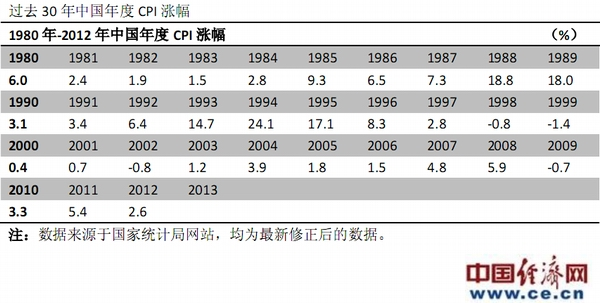
\includegraphics[width=\linewidth]{tongpeng30.jpg}
  \caption[1980--2012年CPI通膨率]{\label{fig:tongpeng30}注:图中CPI涨幅为本年相较
    上一年的涨幅。 }
  \capsource{\url{http://intl.ce.cn/specials/zxxx/201308/09/t20130809_24648757.shtml}}
\end{figure}

截止到1988年价格闯关前,通货膨胀所收取的高额铸币暗税;1985--1987一些社会事件;
粮食合同定购农民积极性持续下滑,以至于发展到1990年国家要实行强制性更强的“国
家定购”才能完成中央收购;尽快双轨并轨为市场一轨,实行激进“物价、价格闯
关”的主因——“双轨制价格造成的腐败和经济秩序混乱”,也被他们无视掉
了;1988年人民恐慌挤兑抢购的事实何在?只是因为“激进的”价格闯关来临,就没有
之前“温和的”价格双轨制所造成的原因吗?张维迎、张曙光等对双轨制的辩护中,他
们认为计划轨的失败本就属于双轨制改革的目的,那么主要在计划轨上生活的民众怎么
办呢?他们居然说这是无损于弱势一方福利的帕累托改进!

第三,理论方面,帕累托改进局限在哪里?现实中真的会有一方利益无损而另一方利益可以尽
情增长的帕累托改进吗,它是真命题吗?笔者对经济学并不了解,以相当轻率和主
观臆测的态度找到几篇论文,供读者阅读:价格双规制中帕累托改进的理论错误:张军
《价格双轨制:是奇迹还是神
话》\footnote{\url{http://economics.efnchina.com/show-1554-58760-1.html}};帕累托改进的各
方局限性:姚洋《作为一种分配正义原则的帕累托改进》\cite{yaoyang};帕累托改进理论
的伪命题:朱富强《帕累托改进原则能否应用于社会改革?——实践的可行性和内在的
保守性》\cite{zhufuqiang},宋圭武《“帕累托最优”质疑》\cite{songguiwu}。

另外,阶段性的帕累托改进形成的发展不平衡、财富分化往往会为下一次经济下行期带
来较大矛盾和压力。此一阶段的成功,可能是下一阶段大萧条的根源所在。

更大胆来说,帕累托改进本身就是一个伪命题。人类社会是互相动态联系的整体,拔高一极,
另一极不变,无可辩驳地会造成拔高一方对不变一方的权力压制。这本是中二生依据自
己的现实经验就可以明白的道理,无需什么旁征博引。

第四,也是最后一条。双轨制的发明被认为是1984年莫干山会议的重大成果。这次会议
参会者是通过征文入选,投稿人多是在读硕士研究生、讲师等青年人。参会者就“究
竟谁最早提出双轨制”的争论;也有石油系统或其他公司认为自己早在80年代之初便已
实际实施双轨制,应是双轨制发起人。笔者妄断,其实这都不重要,双轨制的路径是预
设的,莫干山会议只是作为批判的武器或曰喉舌——为双轨制增加经济学份量的一次会议。


据国际货币基金组织《国际金融统计》和数据文件,1987年CPI通胀率较上年上
升7.234\%,1988年较上一年上升18.812\%,1989年较上一年上升18.246\%。

杨继绳\cite{yangshuanggui}和张曙光就李鹏向邓小平反映价格问题的时间有出入,杨继绳
说是七届全国人大一次会议期间,张曙光说是两会后,笔者认为并没有实质的差别,以下以
张曙光记述为准。
\begin{quotation}
  1988年3月25日到4月13日,一年一度的“两会”在北京召开,\textbf{物价和“官倒”}问题成为会
  议议论的焦点。代表们强烈抨击双轨制给不法分子可乘之机,痛斥社会风气每况愈下。

  两会后,李鹏向邓小平汇报会议情况。邓小平问代表们意见最大的是什么事情,李鹏说是
  价格问题,\textbf{双轨价格造成的腐败和经济秩序混乱}。邓小平再次提出要闯过价格改革这一关。
  并认为“\textbf{晚过不如早过}”、“\textbf{长痛不如短痛}”。事后,李鹏向中央政
  治局传达了邓小平价格闯关的意见。\pagescite[][563]{fengyunshi1b}
\end{quotation}

1988年8月15日至17日,中共中央政治局在北戴河召开第十次全体会议,通过了《关于价
格、工资改革的初步方案》,\textbf{价格闯关正式开始,部分烟酒市场价较原来提高10倍,
  全国挤兑抢购现象相当严重。1989年2月,CPI通胀率同比(去1988年2月相比)增
  长28.4\%,为改革开放以来同比最高比例。}

1988年因价格闯关彻底失败,保守派势力处于上升趋势,自由派势力相当之前有所减弱。
同年9月26日至30日,中共十三届三中全会召开,“会议批准了中央政治局向这次全会提
出的\textbf{治理经济环境、整顿经济秩序、全面深化改革}的指导方针和政策、措施。……治
理经济环境,主要是压缩社会总需求,抑制通货膨胀。整顿经济秩序,就是要整顿目前
经济生活中特别是流通领域中出现的各种混乱现
象。
”\footnote{\url{http://cpc.people.com.cn/GB/64162/64165/70293/70319/4857100.html}}

\begin{quotation}
  由于连续两年的治理整顿,再加上1989年的政治风波,中国的经济运行发生了重大变化,
  从经济过热变成增长过慢,从通货膨胀变成通货紧缩。1988年和1989年GDP分别增
  长4.1\%和3.8\%,1990年和1991年零售物价上涨率从1988年的18.5\%和1989年的17.8\%下
  降到1990年的2.1\%和1991年的2.9\%。市场秩序也发生了逆转,从紧张变成疲软,从旺销
  变成滞销,持续了几十年的卖方市场第一次出现了买方市场,这就导致了计划内外价差的
  缩小,计划价格变成了市场价格。于是,双规价格自然而然地实现了并轨,到1991年底,
  80\%的商品价格都已经放开,基本上实现了市场化。这真是“踏遍铁鞋无觅处,得来全不
  费功夫”。\pagescite[][579]{fengyunshi1b}
\end{quotation}

笔者想,一些领导人和西方主流经济学家极力推动,举国之力想要完成的事情都没有完
成,却被历史和真正市场(并非现代西方经济学所说的“自由”市场)以一种荒谬、戏
谑众生和神奇的自我动态平衡实现了最终的并轨……


\section{金融改革}
\label{sec:huilv78}

\subsection{现代化银行}

1979年10月4日,邓小平同志在省、自治区、直辖市党委第一书记座谈会上作出讲话,收录在
《关于经济工作的几点意见》。意见中指出:“必须把银行真正办成银行……过去我们的制
度是采取拨款的形式,而不是银行贷款的形式。这个制度必须改革。任何单位要取得物资,
要从银行贷款,都要付利息。”我国开始了恢复、重构金融体系的工作。

1979年到1984年,中国恢复和建立了中国农业银行、中国银行、中国建设银行等专业银
行;中央人民银行专门行使中央银行职能;成立中国工商银行,承担原来由人民银行办
理的工商信贷和储蓄业务。同期也成立了中国国际信托投资公司和地方信托投资公司、
租赁公司、农村和城市信用合作社等。

1985年后,中央政府按照市场化运作的原则成立了一批股份制商业银行,包括交通银行、中
信实业银行、华夏银行等。

1986年12月19日,邓小平同志在听取中央负责同志汇报时再次指出“要把银行真正办成银行。
我们过去的银行是货币发行公司,是金库,不是真正的银行。对金融问题,我们知识不足,
可以聘请外国专家做顾问嘛”。

1995年《中国人民银行法》公布以前,财政部可以向人民银行借款和透支,用于弥补中
央财政赤字和解决专项支出。《中国人民银行法》关于“中国人民银行不得对政府财政
透支,不得直接认购、包销国债和其他政府债券”的规定出台后,中央财政不能再从人
民银行借款。同时《预算法》规定政府财政赤字只能通过发行国债来弥补。

\subsection{汇率双轨制}

杨帆将市场经济过渡时期的汇率制度变革分为两个阶段。\cite{huilvshi}

20世纪70年代后期,因人民币汇率被严重高估,\textbf{全国平均出口换汇成本
  较官方汇率过高,造成企业出口越多亏损越大。}笔者根据杨帆文中表格测
算,1975--1979年的出口平均换汇成本均高于同期官方汇率50\%以上,最高达至68\%。

1978年8月为促进出口,平衡外汇收支,我国开始实行\textbf{外汇留成制},所谓“外汇留
成,即是对外贸易单位和出口生产企业把收入的外汇卖给国家,国家按一定比例拨给他们相
应的外汇留成。”

\begin{quotation}
  “外汇留成有两种形式,一种是\textbf{现汇}(在企业和地方、国家间直接分配外汇数量),一
  种是\textbf{额度};且以后者为主。所谓外汇额度,是指按照官方汇率获取外汇的一种权
  利。其目的是\textbf{政府直接控制外汇},其办法是,外贸企业必须将\textbf{包括留成
    外汇在内的全部收汇,按官方价格售给政府指定的银行,}同时按照留成比例拿到一个凭
  证,即\textbf{外汇额度}。当该企业想使用外汇时,再持\textbf{外汇额度凭证}到银行
  按照政府规定的汇率用人民币购买外汇”。\pagescite[][769]{fengyunshi1b}
\end{quotation}


杨帆将1981年至1984年间划分为转轨时期第一阶段——“\textbf{人民币内部结算价和官方汇
  率并存的双重汇率时期}”。此一时期,\textbf{贸易内部结算价}基本不变,“内部结算价
按照1978年全国平均换汇成本2.53人民币/美元加上\textbf{10\%的出口利润}计算出来,
为2.8人民币/美元……我国贸易收支明显好转,外汇储备明显增加。\textbf{1984年外汇储备
  年末累计余额170.42亿元特别提款权,为历史上和20世纪80年代最高水平”}。

\begin{quotation}
  有外汇额度的企业暂时不用,而没有外汇额度的企业却急需用汇,外汇额度交易
  (\textbf{合法和非法})及其交易场所就应运而生。\pagescite[][769]{fengyunshi1b}
\end{quotation}

1980年到1983年中国银行先后在北京、上海等12个城市开办了外汇调剂业务。张曙光指
出,\textbf{调剂柜台外汇交易价格}为贸易内部结算价2.8人民币/美元基础上上
浮10\%,3.08人民币/美元),但这仍然低于\textbf{市场实际成交价格}。

\begin{quotation}
  随着外汇留成的增加和官方控制的放松,\textbf{私下的场外交易}发展起来……一美元可以
  兑付4--5元人民币。这样,外汇额度的价值已经由\textbf{市场}来评价了。\textbf{一般的交易方
    式}是,(笔者注:有外汇或外汇额度凭证的企业)先在银行按照官价提取外汇,出
  门后再按\textbf{黑市价格}补齐(笔者注:按黑市价格卖给需求外汇的企业或个人
  )。\pagescite[][769]{fengyunshi1b}
\end{quotation}

杨帆提及“(第一阶段)影响了\textbf{非贸易部门}的积极性……\textbf{外贸亏损增大},在对外
经济中陷入被动,造成了\textbf{外汇管理的混乱},更加重了\textbf{国家的财政负担}。因此实行
内部结算价注定成为一个\textbf{过渡时期的应急措施}。”

杨帆将1985--1993年间划分为转轨时期的第二阶段:
\begin{quotation}
  \textbf{官方汇率}和\textbf{外汇调剂市场汇率}并存时期。 从1985年1月1日起,我
  国\textbf{取消内部结算价},官方汇率应用于\textbf{贸易结算}和\textbf{非贸易外汇
    兑付}。

  为\textbf{鼓励出口},在\textbf{人民币汇率下调}的同时,1985年国家又一
  次\textbf{提高外汇留成比例},采取按出口商品收汇金额比例留成的办法。
\end{quotation}
这一阶段官价实行以美元为基准的有限弹性汇率制。综合来看汇率恰逢其时的步入
了\textbf{实质性和典型的价格“双轨制”时期}。

\begin{quotation}
1988年上海首创外汇调剂公开市场,实行公开竞价制度,其它城市也纷纷效仿。这样一来,
外汇现汇交易和额度交易就\textbf{合法化}了。\pagescite[][769-770]{fengyunshi1b}

1988年后,国家\textbf{放开了外汇调剂价格},调剂价格根据外汇供求\textbf{自由浮动}。
同年,在北京设立了\textbf{全国外汇调剂中心},形成了全国统一的外汇调剂市
场。\cite{wangqiangshehui}

1988年我国外贸体制进行了重大改革,外贸开始推行承包责任制,并对轻工、工艺、服装三
个行业实行独立核算、自负盈亏。1991年外贸由补贴机制转向自负盈亏机制,取消财政补贴。
外贸体制改革的深化,要求人民币汇率成为调节进出口贸易的主要手段。

1988年至1993年由于\textbf{经济过热、通货膨胀}、物价上涨、进口需求猛增\footnote{据管
  涛,1993年,中国出现了历史上最后一次年度贸易逆差。},外汇\textbf{求大于供},市场
汇率\textbf{不断下跌},由5.70人民币/美元贬值为1993年2月的8.20人民币/美元。为了\textbf{限制汇率
  投机性上涨},一度实行限价,造成\textbf{外汇流向场外交易}。1993年5月\textbf{取消限价},
市场汇率骤升至\textbf{11.20人民币/美元}。1993年7月以后,在国家加强宏观调控和中国人
民银行对市场进行干预下,到1993年底市场汇率回落到\textbf{8.72人民
  币/美元}。\cite{huilvshi}人民币市场汇率贬值波动在 43.86\% -- 96.49\%之间。

从1994年1月1日起,国家决定实行\textbf{单一的有管理的浮动汇率制},实现了官方汇率与
调剂市场汇率的并轨。特别要强调的是,1994年汇率并轨时,人民币汇率制度是\textbf{以
  市场供求为基础的、 单一的、有管理的浮动汇率制度}。其中,这个“单一”\textbf{不
  是单一盯住美元的汇率制度},而是相对于1994年并轨以前的双重汇率制度来说的。双重汇
率制度时期,官方汇率和外汇调剂市场汇率的差价很大,并轨以后,所有的交易都使用
了\textbf{市场形成的汇率},因此,强调了“\textbf{单一}”。\cite{guantaohuigai}
\end{quotation}

1月1日汇率强行并轨,从5.8贬至8.72,一次性贬值50\%,全国通货膨胀率24\%.

市场经济体制过渡时期的汇率双轨思路是一贯的,国家抛弃财政包袱,减少对各方面投
入和支持,获取收益,解决原来企业出口亏损问题,通过汇率双轨、特别是持续增加市
场一轨的权重刺激出口,做大市场。

\begin{quotation}
  双轨并轨使中国贸易顺差持续加大,促进了中国国内分工的深化和商品经济的繁荣;
  但与此同时,也令中国丧失了货币主权。\textbf{顺差依赖}成为中国经济的阿喀琉斯之踵,
  美联储利率的波动成为人民币信用震荡的主要外源。\cite{dajueqi}
\end{quotation}

改革过程中出现的问题也是简明的,同农业、企业方面的双轨制一样,其中市场轨增大
了权利寻租的操作空间,并过来压榨计划轨。双轨制似乎是势在必行的,权力寻租似乎
也是无法避免的。笔者认为,这可能是历史的趋势吧,不以个人或组织(包括国家)主观意
愿为转移的趋势。

但笔者也认为,不管负面影响是不是大势所趋,在任何政策的制定和执行过程中,不能
因为负面影响不可避免,就完全忽视负面,这已经成为一些当代学者和官僚的通
病。\improve[inline]{是不是将结论放到本章结尾再行论述呢?只展示资料?}

\section{财政改革}

\subsection{财政体制改革的深层逻辑}

2008年3月18日,时任国务院总理温家宝在十一届全国人大一次会议的记者见面会上说:“其
实一个国家的财政史是惊心动魄的。如果你读它,会从中看到不仅是经济的发展,而且是社
会的结构和公平正义。”

\begin{quotation}
  回顾40年改革长路,是什么在推动中国财政改革?其深层逻辑又是什么?我们发现,从过
  去到现在,这一问题根本上可以归结为一点,那就是公共风险的变化。\textbf{财政改革
    往往不是在先见之明的制度设计基础上进行的,而是在公共风险暴露与加剧时,不得不
    做出的选择。}

  \textbf{防范和化解公共风险是财政改革的原动力。}从历史上看,制度变迁无一不是公共风
  险与危机推动的结果,而制度变迁的突破口常常是在财政。改革开放以来,我国财政
  改革实质上都是遵循公共风险变化的逻辑而推进的,其变化的脉络是从“\textbf{家贫国
    穷}”的风险到“\textbf{机会不均}”的风险,再到\textbf{全球公共风险},这也是我国主要公
  共风险的昨天、今天和明天。\cite{cai40}
\end{quotation}

\begin{quotation}
  1978年12月中共十一届三中全会的改革开放,提出解放思想。理论界批评投资饥渴症,
  提出要扩大企业自主权,强化对企业的预算约束,让企业成为独立的经济核算单位,
  自负盈亏。对应的改革,一个是“\textbf{利改税}”,即把企业向国家财政纳税和上交利润
  两种形式,改为只向国家纳税一种形式。另一个是“\textbf{拨改贷”},即把基本建设投资
  的财政拨款改为由企业向建设银行贷款,项目建成投产后,还本付息。\cite{bogaidai30}
\end{quotation}

\subsection{财政包干制}

据《央地关系》:
\begin{quotation}
  从80年代初到90年代中期,中国改革的主要手段就是\textbf{承包制},所谓“\textbf{一包就
    灵}”,是适用于整个80年代的总体改革思路。承包制从农村开始,逐步扩展到企业
  以至于中央地方关系领域。

  我国自1980年就开始试行财政承包制,经过几次尝试,到1988年在全国推行开
  来。\textbf{财政承包},其基本思路是中央对各省级财政单位的财政收入和支出进行包干,
  地方增收的部分可以按一定比例留下自用,对收入下降导致的收不抵支则减少或者不
  予补助。这与农村包产到户与企业承包制的方法是基本一致的。

  财政包干制则更加接近于真正意义上的中央对地方的“分权”。包干制总的精神就
  是“包”,“包”的前提就是将中央和地方各自的收支权限划分清楚,中央“包”给
  地方的是\textbf{收支总数},而不对地方的增收、减支的权利多加干预。这种“一揽子”包
  干实际上赋予了地方政府相对稳定的配置物资、管理企业的权限,地方政府开始逐步
  变成有明确的利益和主体意识的单位,而不再是被“条条”系统不断分割的、相对零
  散的“块块”。
\end{quotation}

1980年2月,国务院颁发了《关于实行"\textbf{划分收支,分级包干}"的财政管理体制的规
定》,划分中央和地方财政的收支范围;对于15省确定包干基数,基数以外收入中央和
地方比例分成;扩大地方财政权限,中央各主管部门对于应对由地方安排
的各项生产建设和文教事业,不再归口按“条条”安排支出,不再向地方分配财政支出
指标”,“\textbf{原则上五年不变}”。俗称“\textbf{分灶吃饭}”,改变了过去“统收统支”的
财政体制。\improve[inline]{historychina 好像没有介绍总额分成的含义?}

\begin{quotation}
  但是自1981年起,因为中央的财政收入下降,就开始着手\textbf{改变}这种“分级包干”的办
  法。到1982年6月底,在上述15个省份中,有10个又回到了“\textbf{总额分成}”的办法;
  到1983年,15个省份就全部恢复了“总额分成”的办法,分级包干的尝试可以说是名
  存实亡。

  唯一留下的改变是广东和福建两省实行的“\textbf{大包干}”财政体制。所谓“大包干”,
  其关键在于由比例上解和比例补助变为\textbf{定额上解}和\textbf{定额补助},其中广东实行的
  是定额上解,收小于支的福建实行的是定额补助。定额上解和定额补助的含义就是超
  基数部分100\%归地方所有,中央不再分享超收部分。广东、福建实行的定额包干体制
  一直没有改变,可以算作中央推行\textbf{定额包干的试点省份}。

  在这个阶段(1985--1987年包干制的过渡阶段),中央和地方实行的包干体制可以概括
  为“\textbf{划分税种,核定收支,分级包干}”。在此期间,全国17个省级单位仍然与中央
  实行\textbf{总额分成}的体制,但是与此前一年一变的总额分成体制相比发生了一个重要的
  变化,就是\textbf{分成比例固定下来并且一定五年不变。一定五年不变,实际上为地方财
    政增收提供了动力。}其中,黑龙江与广东一样,实行定额上解的“大包干”办法,
  超收部分上解额度是0.65亿元。另外,吉林、江西、陕西、甘肃、湖北、四川也开始
  与福建一样,实行\textbf{定额补助}的办法。这样,定额包干的省份由第一阶段的2个增加
  到7个。其他少数民族和边疆省份则实行\textbf{民族地区预算管理体制},实际上也是\textbf{定
    额补助}体制。\cite{yangdi}

  (1988—1993年包干制的全面推行阶段)是比较彻底的所谓“\textbf{分灶吃饭}”的财政体制
  阶段。在这个阶段,包干形式多种多样,全国39个省级单位(省、自治区、直辖市和
  计划单列市)共实行了六种不同的包干形式。

  包干制将地方的经济发展速度与地方政府的财政收入挂钩,使得地方政府为了增加财
  政收入,就要提高地方经济发展速度。随着实行大包干的省份越来越多,地方政府之
  间也就经济发展展开了\textbf{区域间的竞争}……这就是财政分权导致的地方政府“\textbf{放水
    养鱼}”的竞争模式。

  在地方政府的各层级内,也普遍实行了中央与省级政府的包干制。


  从理论而言,这个体制体现出的是一种与企业管理类似的激励模式。这正是戴慕珍提
  出的“\textbf{地方国家公司主义}”的微观运行机制的核心,是\textbf{地方政府“公司化”}的
  主要动力之一。在地方的实践中,乡镇政府要实现自己可支配收入的最大化,并非一
  味地以收入最大化为目标。因为在这种包干制下,在一个体制周期内收入的快速增长
  会提高下一周期内的收入基数和收入任务数,这会增加下一体制周期内完成任务的难
  度,并造成自身收入的减少。因此,乡镇政府的行为策略是应该与乡镇政府官员的任
  期制结合在一起理解的。如果一个官员为了博取很快的晋升,他可能会尽全力增加其
  任期内的财政收入;如果一个官员预期到自己会在相当长的一段时间内留在本乡镇,
  则他可能会对收入增长的速度进行适度的“控制”。而对于县级政府来说,这种周期
  性的对基数和任务数的调整使得在增加乡镇增收激励的同时,又能保证县级财政的收
  入不会大幅度减少,并且会在下一周期内实现快速的增长。另外,通过调节超收分成
  的比例,县级政府可以对增收较快和较慢的乡镇进行刺激,比如通过加大留成比例,
  就可以鼓励乡镇多超收;通过缩减这个比例,又可以在一定程度上集中乡镇的收入或
  者“劫富济贫”。
\end{quotation}

\subsection{税制改革}

1980年9月10日,第五届全国人民代表大会第三次会议通过了《中华人民共和国中外合资
经营企业所得税法》和《中华人民共和国个人所得税法》。1981年12月13日,第五届全
国人民代表大会第四次会议通过了《中华人民共和国外国企业所得税法》。中国\textbf{涉外
  税制}初步建立。

为理顺中央与地方、政府与企业的分配关系,政企分开、增强经济活力,“使企业真正
成为自主经营、自负盈亏、自我发展、自我约束的商品生产者与经营者,减少政府对企
业的行政干预和条条、块块分割的矛盾,企业对中央与地方只承担纳税的义务”\footnote{田纪
  云《光辉的八十年代》},实现“国家得大头、企业得中头、职工得小头”的目标,中
国开始了利改税。

1983年4月24日,国务院批转财政部制定的《关于国营企业利改税试行办
法》,规定“\textbf{以税代利,税利并存}”,国营企业上交利润转为上交税收,实现了
(\textbf{利改税})的第一步改革,允许企业使用\textbf{税前利润归还银行贷款本息},并且\textbf{小
  型国有企业自负盈亏}。9月18日,国务院批转财政部《关于在国营企业推行利改税第
二步改革的报告》,并颁布了《国营企业第二步利改税试行办法》,规定10月1日 起试
行第二步利改税,进一步分解增设多种税种,由\textbf{税利并存逐步过渡到完全的以税代
  利}。

根据田纪云1984年1月20日《关于完善利改税制度的几个问题》:
\begin{quotation}
  据初步计算,1983年全国实行利改税的国营企业新增加的收入,以税金和利润的形式
  上缴国家的约占\textbf{70%}左右,企业所得约占\textbf{30%}左右,其中用于职工奖励基金的部分约
  为\textbf{8%}左右。

  % 有的同志提出,在社会主义制度下,企业实行“独立核算,自负盈亏”,会不会影响
  % 企业所有制的性质?……既不会改变企业的全民所有制性质,又能使企业这个最基本
  % 的经济细胞增加活力,有利促进生产力的发展。
\end{quotation}


\improve[inline]{从国营企业到国有企业的性质转变是否还要写?}
% 从国营企业的性质变化到国有企业。
 % 1993年3月八届全国人大一次会议通过了宪法修正案,正式将“国营经济”的提法改为“国有经济”,将“国营企业”的提法改为“国有企业”。

1985年3月21日,国务院发布《关于实行“划分税种、核定收支、分级包干”的财政管理
体制的规定》,进一步改革包干式财政管理体制,“\textbf{一定五年不变}”。

国营大中型企业利改税综合税赋约为利润的70\%,税赋较重。\textbf{税前还贷}使中央财政支
出不降反增;经营状况好的企业被\textbf{鞭打快牛},亏损的企业包盈不包亏——亏损算国家
的;一些企业和地方政府两本帐,消极预算内收入(税收),热衷于预算外收入(非税
收入)。

利改税实行一年之后便让位给承包制。\improve[inline]{利改税让位承包制,论述不清,
  有待加强}
\begin{quotation}
  针对两步利改税中暴露出来的\textbf{价格、税收、信贷等宏观体制不配套}的问
  题,1984年-1985年,国家开始酝酿以\textbf{价格、税收、财政为中心的配套改革}。但是,
  这一时期出现了严重的投资、信贷失衡,因此,这一改革方案虽由国务院讨论通过并
  得到中央批准,却最终未能推开。在价格、外汇等方面,采取了\textbf{双轨制}的过渡办法。
  而企业改革的重心则转向推广\textbf{承包制}。\footnote{吴晓灵 《国企改革前奏(1978年-1992年):扩权让利与承包制》}
\end{quotation}


\textbf{税制改革从此成为中央与地方政府的博弈场}。依马骏所说,原“分灶吃饭”税制
中,“20\%共享收入归地方的一刀切计算办法使富省多有结余,穷省多有赤字”,因此
促成了这次改革。新税制改革的弊端是:
\begin{quotation}
  自1978年底以来,政府财政收入占国民生产总值的比例及中央财政收入占全部财政收入的
  比重快速地下降。

  \textbf{(地方政府)利用各种减免税来调节其实际税收}……地方政府对有效税率及税基的
  控制还表现在其对财政收入渠道的控制……\textbf{地方政府预算内收入比重的下降和预算
    外收入上升},中央政府控制全国财政收入与支出的能力相应下降。

  \textbf{由于地方政府在事实上控制了有效税率和税基,中央政府越来越多地依赖于一些不
    规范的政策工具来控制地方向中央上缴的财政收入。}\cite{majuncaigai}
  \improve[inline]{分税制也要借鉴这篇文章}
\end{quotation}

1988年税制改革见下一节。

财政部官网转载刘邦驰、马韵《三十年税制改革的回顾与发展趋
向》
\footnote{\url{https://www.mof.gov.cn/zhuantihuigu/czgg0000_1/czggcz/200811/t20081106_88385.htm}}
,将1978年--1993年这一时期的税制改革称为“有计划商品经济时期的税制改革”,涉
外税制、利改税(“新中国成立后实行了30多年的国营企业向国家上缴利润的制度改为缴
纳企业所得税和调节税”)、个人所得税等税务改革。
\begin{quotation}
  这一时期全面改革了工商税制,建立了涉外税制,彻底摒弃了“非税论”和“税收无
  用论”的观点,恢复和开征了一些新税种,从而使我国税制逐步转化为多税种、多环
  节、多层次的复合税制,税收调节经济的杠杆作用日益加
  强。
  \footnote{\url{http://finance.ce.cn/sub/2013zt/zgszgg/hgyzw/201304/18/t20130418_199980.shtml}}
\end{quotation}

\subsection{拨改贷}
\improve[inline]{http://www.reformdata.org/2008/0916/23089.shtml}

\begin{quotation}
  1979年4月的中央工作会议期间,邓小平在一次省市委第一书记会议上讲了话:是否可
  以设想,\textbf{将财政拨款制度改为银行贷款制度,把银行作为发展经济、革新技术的杠
    杆。}银行应该抓经济,现在只是算账、当会计,没有真正起到银行的作用。对投资
  少、见效快的企业,要采取\textbf{不用财政拨款,而用银行贷款}的办法。\cite{bogaidai30}
\end{quotation}

1985年,所有国家基本建设投资由财政无偿拨款改为向中国人民建设银行贷款,并要还
付本息,即“\textbf{拨改贷}”,信托投资公司也随之兴起。
\begin{quotation}
  实施“拨改贷”的初衷是: 与无偿拨款不同,获得贷款的企业要还本付息,从而促使
  企业精打细算,先用自有资金建设,缩短工期,提高效率,把加速资金周转和提高经
  济效益提上企业的议事日程。

  1984年国家出台拨款改贷款政策后,意味着1984年以后新成立的国企,一出生就
  是\textbf{100\%的负债率}。\cite{bogaidaizhaizhuangu}

  % 国有企业高负债率的直接原因是国家在1983年实行了拨改贷,对国有企业的投资由
  % 财政拨款改为向银行的贷款。国有企业高负债率的间接原因则是国有企业的预算软
  % 约束}。\cite{linyifuzhai}

  银行系统贷给国有企业的贷款很多都成了呆坏账,国有企业拖欠还贷的情况非常严重。
  但是,出于对国有企业进行政策性支持的需要,银行在政府的影响下,会继续向那些
  企业发放贷款。这样日积月累,便形成了银行系统今天巨额的不良资产。(林毅夫与
  李志赟就此总结有三个原因,一是计划经济转入市场经济过程中,原资本密集型国有
  企业尤其受到外资、合资企业冲击,由此造成的\textbf{战略性政策负担};二是国有企业承
  担了大量劳动力的养老、医疗、教育等社会保障责任,由此造成的\textbf{社会性政策负担};
  三是无法划清亏损\textbf{企业经营者的责任},经营者往往将责任归咎于前两者,并以此为
  理由拖欠银行贷款,政府在各方面压力下干预银行,要求银行继续贷款给亏损企业,
  由此造成\textbf{预算软约束}\footnote{软预算约束就是指当一个经济组织遇到财务上的困境时,借助
    外部组织的帮助得以继续生存这样一种经济现象。}问题。)\cite{guoyoujinrong}

  1988年,国家实施税收制度改革,明确了“\textbf{税利分流、税后还贷、税后承包}”政策,
  规定企业债务由税前还贷改为税后还贷,\textbf{原来由财政减税负担一部分还贷责任,改为
  全部要由企业的盈利偿还。}尽管当时限于国有资产的产权制度尚未建立,国家最终没
  有解脱对国有企业承担的无限责任,但是这样一种政策规定,实际上是要\textbf{国有企业代
  替国家完全承担出资者的经济责任,国家成为既未出资,也不对投资经营后果承担责
  任的出资者。}\cite{bogaidai30}
\end{quotation}

银行由财政部门的会计和出纳成为功能健全的现金融商业银行。但此时“利用存款发放
贷款的指标,也要由国家计委分配,变成了按部门归口切块分配投资和贷款”。


\improve[inline]{下一章或可加入《由“拨改贷”到“债转
  股”》\url{http://www.hprc.org.cn/gsyj/jjs/jjyxs/201702/t20170220_388850.html}}

\section{土地财政}

1978年,中国人均住房面积6.7平方米。

1978年1月至1979年2月的一年间,邓小平相继访问了缅甸、尼泊尔、朝鲜、日本、泰国、
马来西亚、新加坡和美国。这一系列出访,特别是对美国、日本、新加坡的访问,奠定
和加强了邓小平自由开放的决心。

1978年9月,中央召开的城市住宅建设会议传达了邓小平同志的一次重要谈话,大体精神
是:解决住房问题能不能路子宽些,譬如允许私人建房或者私建公助,分期付款。把个
人手中的钱动员出来,国家解决材料。建筑业是可以为国家增加收入、增加积累的一个
重要产业部门。在长期规划中,必须把建筑业放在重要位置。

1978年11月的新加坡之行使邓小平对公共住房计划和工业园区感触颇深。
\begin{quotation}
  \textbf{一、公共住房计划}

  邓小平听取了关于公共住房计划情况的介绍,并登上该局22层办公大厦的顶层,瞭望
  周围一幢幢新建成的公共组屋。小平询问了新加坡每年住房建筑的总面积和其他有关
  问题,在得悉新加坡总共有三万名技术人员和工人从事住房建筑的情况之后,他说,
  新加坡的建筑机械化程度高。

  据中国新闻社报道,结束访问新加坡之后,12月2日,邓小平约胡耀邦、胡乔木、于光
  远等在家中谈话,特别举了新加坡的例子:新加坡月收人1500新币有权买房产,五房
  单位,70平米,花半年工资。那里的房租是工资的15\%,而欧美日则是三分之一。

  \textbf{二、工业园区}

  邓小平也到裕廊工业区,听取了相关介绍,并登上五层楼高的瞭望塔,鸟瞰这个新加
  坡最大的工业区。新加坡以裕廊工业区为基地,提出面向出口的工业化战略,走跨国
  公司投资为主的发展道路。时至今日,裕廊工业区依然保持着旺盛的活力,其发展模
  式是中国各地的开发区借鉴的对象。

  李光耀向邓小平介绍了外商投资对新加坡的好处。邓小平回忆说:“我到新加坡去,
  了解他们利用外资的一些情况。外国人在新加坡设厂,新加坡得到几个好处……我们
  要下这么个决心,权衡利弊、算清账,略微吃点亏也干。” \footnote{新加坡眼
    《\href{https://www.yan.sg/gaibianeshijiegejucbxiaopige/}{45年前的今天,
      新加坡迎来了邓小平;他的改革开放,改变了世界格局}》}
\end{quotation}

据赵燕菁\cite{dajueqi}:
\begin{quotation}
  1979年3月,骆锦星调职深圳担任深圳市房管局副局长。征得时任省委书记任仲夷的许
  可后,他选择了通过贸易补偿,获取地产开发资金——\textbf{港商刘天就出钱,特区政府出
  地,建房子到香港卖},对于收入,深圳市政府和刘天就按85:15分成。为了吸引香港购
  房者,允许“一次性付款9.5折,提供购房入户,每家配备3个户口名额”,价格比香
  港的便宜一半。这一政策刺激了在内地有亲属的香港居民的购房欲望,结果楼盘很快
  售罄。\textbf{中国第一个商品房小区}——\textbf{东湖丽苑}出现了。这就是最早的“\textbf{土地财政}”的雏
  形。骆锦星后来回忆说:“东湖丽苑是土地商品化的体现,开了土地有偿使用的先
  河。”此后,很多香港房地产开发商来深圳要求合作,深圳意识到了土地的价值。
\end{quotation}

据骆锦星回忆,彼时深圳基建较落后,资金短缺,当时规划建设罗湖小区,造价3亿,国
家贷款给3000万,剩余缺口2.7亿由深圳想办法。1979年8月深圳房管局提出以“\textbf{土地
  使用费}”解决城市建设资金难题。小区由外商独资,以1∶10的容积率建设,即1平方
米土地建设10平方米的高楼。一平方米收\textbf{5000元土地使用费},合同签订后要
交50\%,\textbf{卖楼花}后交齐。项目出租5块地,占地1.1平方千米,收回5亿多元资金。

源于香港,始于深圳,自此拉开中国土地财政序幕。赵燕菁认为:
\begin{quotation}
  开发和建设深圳的故事显示,并不是只要有经济活动,就会自发形成基础设施;而是
  要政府先提供基础设施,才能招商引资。\textbf{基础设施建设资金来自土地收入,其价值
    体现的是未来城市“外部性”带来的现金流的贴现。}没有“土地财政”,深圳
  的“第一动力”就不会产生。中国城市化伟大成就背后的重要原因,就是创造性地发
  展出一套\textbf{将土地作为信用基础}的制度——“\textbf{土地财政}”,也正因如此,\textbf{“土
    地财政”乃是一种金融活动。将土地收入视作“财政收入”,暴露出传统经济理论
    对真实世界的错误观察和认识。}

  只有政府提供了重资产(笔者注:企业不愿投入的、耗资巨大、长周期、低回报等难
  见市场效益的公共(产品)服务\improve[inline]{需整理语句,可根据《大崛
    起》。}),其他社会主体才可能以轻资产启动各类商业模式。\textbf{城市化就是资本不
    断聚集的过程}。
\end{quotation}

根据王永红《攀登新的高度——我国土地有偿使用制度改革30年历程》:
\begin{quotation}
  \textbf{1. 启用经济杠杆,土地由无偿、无期限、无流动向有偿、有期限、有流动转变}

  1979年7月五届全国人大二次会议审议通过和颁布施行的《中外合资经营企业法》规定,
  可以\textbf{出租批租}土地给外商使用。

  同年12月31日,成立不久的广东省深圳市,签订了\textbf{第一个吸引外资开发经营房地产项
    目合同},由深方提供土地,香港妙丽集团投入资金,合作兴建和经营住宅楼,规定税
  后纯利深方、港方按85∶15分成。

  (笔者附:1980 年 9 月北京城市开发总公司成立。同年12月9日国务院批转《全国城
  市规划工作会议纪要》,提出可以组织开发公司,对土地进行综合开发。1981 年 1
  月,中国房地产开发集团公司由国务院批准组建,这是中国第一家房地产开发公司,
  房地产项目从此开始出现。)

  由于合作经营很成功,妙丽集团进而申请独资开发经营。1981年2月,双方签订合同,
  深圳市提供6000平方米“\textbf{地皮使用权}”,由妙丽集团“独资兴建和经营商住大厦”,
  土地使用年期30年,使用费每平方米5000港元。至1981年12月的两年间,深圳房地产
  公司单在罗湖小区就“引进外商独资经营房地产项目10个,订租(出租)土地4.54万
  平方米,土地使用费21360万港元;另有8.1万平方米土地作为4亿多港元的物化资本,
  在10个项目中与外商6亿多港元的投资合作建造商品楼宇”,“使昔日杂草丛生的罗湖
  小区,很快变成了高楼林立的商业、金融中心”。

  《深圳经济特区土地管理暂行规定》自1982年1月1日起施行,规定了不同用途土地各自
  使用最长年期和不同用途不同地区每年每平方米土地使用费标准。还规定,土地使用
  费“可一次性付款……也可分年付款,按年息八厘加收利息。”《暂行规定》“适用于
  在特区兴办企业、事业的所有单位”。

  (笔者附:1982年宪法增加“城市的土地属于\textbf{国家所有}。农村和城市郊区的土地,
  除由法律规定属于国家所有的以外,属于\textbf{集体所有};宅基地和自留地、自留山,也
  属于\textbf{集体所有}。”集体所有影响至今,在征收集体所有土地、新增建设用地和拆迁中
  发挥重要作用。)

  辽宁省抚顺市自1984年1月起开征土地使用费,是非沿海城市中起步最早的。开征的缘起
  是,当时的抚顺市主管副市长刘文甲,于1983年听了中共中央党校教授易之关于社会主
  义社会地租仍然存在、城市土地理应有偿使用的专题讲课后,开始琢磨并组织调研,提
  出开征方案。后经市政府讨论通过和财政部批准,全面开征城市土地使用费。尽管当时
  市里还没有“三资”企业,但开征当年就收取土地使用费1300多万元,不仅使城市基础
  设施投资短缺的情况有所缓解,而且有的企业主动退出超占及闲置的土地。至1985年底,
  全市共退还土地15万平方米。

  1984年初,上海市城市经济研究会成立了“上海城市土地有偿使用”课题组,对有偿用
  地的收费形式、方法和标准等六个方面作了专门研究,抽样调查了区位反映最敏感
  的1161家独立核算的商业企业(占全市商业总数的20\%)的土地收益情况。经测算,并
  参考历史上地价水平,将市区用地按地段繁华和开发程度分成7级,郊区、县分为3级,
  设计了3套土地使用费方案。

  广东省广州市自1984年下半年起开征经济技术开发区、新建项目、“三资”项目的土地
  使用费。据介绍,广州城市建设资金每年约需5亿元,但实际只有一半左右,缺口很大,
  征收土地使用费对缓解资金短缺起到了不小的作用。

  1984年下半年,浙江省苍南县龙港镇政府顺应农民盼望进城改善居住条件和从事经济活
  动的愿望,有偿提供土地,成为我国\textbf{第一座农民城}。至1985年底,龙港镇政府收取土
  地使用费1000多万元。后来的12年间,龙港新城建设共投入资金12亿多元,其中90\%是
  通过土地有偿使用筹措的。

  \textbf{收取城镇土地使用费,尽管标准较低,土地仍然由行政划拨,还不能名正言顺地进行市
    场流通,但这一创造性的实践,使原本不值钱、随意使用的土地一下子有了“身价”,
    为我国土地使用制度改革取得历史性突破作好了准备。}

  \textbf{2. 引入竞争机制,从深圳土地拍卖“第一槌”到全面推行经营性用地和工业用地招拍挂出让}

  1987年9月9日,深圳市政府首次以\textbf{协议}方式将一块5321平方米住宅用地的使用权,
  以106万元的价格出让给某公司,使用年限为50年。同年12月1日,深圳市\textbf{首次公开
    拍卖土地使用权},一宗面积为8588平方米的土地被一家房地产公司以525万元的价
  格竞得使用权。这一改革举措面临的最大困境是“违宪”,因为《宪法》明文规定土
  地不能出租、转让。一槌定乾坤。次年4月,《宪法》增加了“\textbf{土地的使用权可以依
    照法律的规定转让}”的条文\footnote{宪法第十条第四款“任何组织或者个人不得侵占、
    买卖、出租或者以其他形式非法转让土地。 ”修改为:“任何组织或者个人不得侵
    占、买卖或者以其他形式非法转让土地。 土地的使用权可以依照法律的规定转
    让。”}。随后,《土地管理法》也作了相应的修改。


  引入竞争机制之路并非坦途,土地拍卖槌声一度相当寥落。有的地方原来已经建立了
  成熟的土地拍卖制度,这时也改为协议出让。\textbf{在协议出让的情况下,关系好的或者
    付了“寻租”成本的人,就能用很低的价格批到好地,国有土地资产大量流失。}
\end{quotation}

一直到二十一世纪初,协议出让仍是土地流转主流,滋生较大权力寻租空间。

1988年8月召开的第一次全国住房制度改革工作会议,明确提出我国城镇住房制度改革的
目标是实现住房商品化,由此进入\textbf{福利住房与市场化双轨}推进时期。

\section{权力寻租、官倒和腐败}

1980年12月26日,陈云在中央工作会议上作报告《经济形势与经验教训》,认为改革步
子要稳缓,谨慎使用外债,财政紧缩,减少基建投资和财政赤字,稳定物价,认清国内
经济基础薄弱,

1981年1月7日,国务院《关于加强市场管理、打击投机倒把、走私贩私活动的指示》
1982年4月10日政治局会议讨论《中共中央、国务院关于打击经济领域中严重犯罪活动的
决定》。4月13日,中共中央、国务院发布了《关于打击经济领域中严重犯罪活动的决定》。
1983年9月15日,人民日报发表评论员文章《必须依法从重从快惩处经济罪犯》。1983年
月12日,中共第十二次全国代表大会发出《中共中央关于整党的决定》。1984年12月3日,
中共中央、国务院发出《关于严禁党政机关和党政干部经商、办企业的决定》。1985年5月
23日,中共中央、国务院发出《关于禁止领导干部的子女、配偶经商的决定》。1986年2月
日,中共中央、国务院发布《关于进一步制止党政机关和党政干部经商、办企业的决定》。
1989年2月5日,中共中央办公厅、国务院办公厅发出《关于清理党和国家机关干部在公司
(企业)兼职有关问题的通知》。

关于价格双轨制时期的权力寻租和腐败论述请见\cref{sec:qishuanggui}。

% 1983年8月,全国政法工作会议公布《中共中央关于严厉打击刑事犯罪活动的决定》,全
% 国从重从速严打刑事犯罪。

改革开放之后,权力寻租和腐败问题普遍发生,贯穿这一时期始终,并未得到有效治理。
有专家学者认为主因是这一时期价格双轨制、利改税、拨改贷等政策的巨大负面作用。
个别专家认为正是改革开放实际实行的体制产生了权力失控,从而导致权贵资本主义的
形成和腐败……比如孙立平\cite{sunlipingkuibai}、钱理群\cite{maohehoumao2}等。


% \begin{verbatim}
% https://www.modernchinastudies.org/us/issues/past-issues/45-mcs-1995-issue-1/253-2011-12-29-11-30-06.html
% 中央与地方财政关系的改革

% 南方周末:重议分税制——分钱还是分权? https://www.guancha.cn/economy/2013_08_15_165993.shtml

% 分税制的是与非 http://liushangxi.blog.caixin.com/archives/60712

% http://www.sss.net.cn/112/65928.aspx
% 刘尚希:财政改革四十年的深层逻辑

% 回顾40年改革长路,是什么在推动中国财政改革?其深层逻辑又是什么?我们发现,从过去到现在,这一问题根本上可以归结为一点,那就是公共风险的变化。财政改革往往不是在先见之明的制度设计基础上进行的,而是在公共风险暴露与加剧时,不得不做出的选择。

%  防范和化解公共风险是财政改革的原动力。从历史上看,制度变迁无一不是公共风险与危机推动的结果,而制度变迁的突破口常常是在财政。改革开放以来,我国财政改革实质上都是遵循公共风险变化的逻辑而推进的,其变化的脉络是从“家贫国穷”的风险到“机会不均”的风险,再到全球公共风险,这也是我国主要公共风险的昨天、今天和明天。

% http://www.cssn.cn/zx/bwyc/201806/t20180626_4421303.shtml
% 中央、地方与企业:财政体制改革40年

% http://theory.people.com.cn/GB/49154/49155/8094994.html

% http://www.pkulaw.cn/fax/czf/contents/class02_3_1r.htm

% http://www.hprc.org.cn/gsyj/jjs/jjyxs/201702/P020170220376223183282.pdf
% 贷改投

% http://www.ccswf.org.tw/files/7100/18/%E5%AD%90%E9%A1%8C3-2%E8%94%A1%E7%A6%BE.pdf

% https://www.guancha.cn/HuAnGang/2014_04_27_224728.shtml
% 分税制改革二十年后

% 建国以来最高通货膨胀是什么时候?
% 19 9 4 年物价 上 涨超 过 2 0 \% , 成为 改革 以来通 货膨 胀 最严 重 的年份
% . 市
% http://img.bimba.pku.edu.cn/res/download/ceq/1_4/010405.pdf

% http://www.chinagrain.cn/axfwnh/2018/09/19/1511534741.shtml
% 我国粮食收储体制改革的历程、体制性问题分析及改革的方向与对策建议

% http://www.china.com.cn/chinese/EC-c/50868.htm  重要粮食流通体制改革:双轨过渡与双轨终结
% \end{verbatim}

% ( 4) 共产主义社会高级阶段。 中国共产党第十三次全国代表大会的报告中指出, 社会主义初级阶% 段 “ 不是泛指任何国家进入社会主义社会都会经历的起始阶段, 而是特指我国在生产力落后、 商品% 经济不发达条件下建设社会主义必然要经历的特定阶段 。” [6 ] % 发达资本主义国家在无产阶级夺取 出自《正确认识和对待“共产主义渺茫论”》
% \improve[inline]{\url{http://theory.people.com.cn/GB/148980/16813293.html},邓小
%   平南巡的三个坚定不移。}


%%% Local Variables:
%%% mode: latex
%%% TeX-master: "../main"
%%% End:
